% Informe final a entregar: Entregable 1 + propuesta, cronograma, presupuesto,
% riesgos, indicadores y avance de las semanas 1 a 6 (con la retroalimentación del asesor)
\documentclass[11pt,a4paper]{article}
\usepackage[spanish,es-noshorthands,es-tabla]{babel}
\usepackage[utf8]{inputenc}
\usepackage[T1]{fontenc}
\usepackage{lmodern}
\usepackage[margin=2.5cm]{geometry}
\usepackage{graphicx,booktabs,tabularx,array,amsmath,amssymb,multirow,longtable}
\usepackage[table]{xcolor}
\usepackage{enumitem}
\usepackage{float}
\usepackage[hidelinks]{hyperref}
\graphicspath{{figuras/}}
\setlength{\parindent}{1.5em}
\setlength{\parskip}{0.4em}
\newcolumntype{L}[1]{>{\raggedright\arraybackslash}p{#1}}
\newcolumntype{Y}{>{\raggedright\arraybackslash}X}
\renewcommand{\arraystretch}{1.15}
\newcommand{\segun}[2]{\iffinal#2\else#1\fi}
\usepackage{algorithm}
\usepackage{algpseudocode}
\floatname{algorithm}{Algoritmo}
\algrenewcommand\algorithmicrequire{\textbf{Entrada}\enspace}
\algrenewcommand\algorithmicensure{\textbf{Salida}\enspace}
\algrenewcommand\algorithmicfor{\textbf{para}}
\algrenewcommand\algorithmicforall{\textbf{para cada}}
\algrenewcommand\algorithmicdo{\textbf{hacer}}
\algrenewcommand\algorithmicif{\textbf{si}}
\algrenewcommand\algorithmicthen{\textbf{entonces}}
\algrenewcommand\algorithmicelse{\textbf{si no}}
\algrenewcommand\algorithmicend{\textbf{fin}}
\algrenewcommand\algorithmicreturn{\textbf{devolver}}
\algrenewcommand{\algorithmiccomment}[1]{\hfill\textit{#1}}

\newif\iffinal
\finaltrue
\newcommand{\EntregableTitulo}{Informe de avance}
\newcommand{\FechaInforme}{4 de octubre de 2026}
\newcommand{\ResumenInforme}{Bimbo despacha a 61 tiendas Bembos lo que el sistema de compras del cliente le indica, sin ninguna validación previa de que esa cantidad tenga sentido. Cuando la tienda se equivoca al registrar el pedido, el error se convierte en producto despachado. Este informe delimita ese problema sobre 10\,374 líneas de pedido vigentes y propone un software que compare cada pedido con el historial de su tienda y explique por qué lo marca. Tras comparar cuatro alternativas, se selecciona la validación con el historial por ser la única que no requiere cambios en el cliente y que permite justificar cada alerta. Se presentan la estructura del trabajo, el cronograma, un presupuesto preliminar de S/~5\,256 con reservas, los riesgos y los indicadores del proyecto. El avance de las semanas 1 a 6 incluye un prototipo que procesa el archivo original y mide reglas sencillas. Con información de semanas completas, la mejor regla acierta en el 45\,\% de sus alertas; al limitarla a lo que se sabe en el momento de alertar, como recomendó el asesor, ese valor cae a entre 6\,\% y 17\,\%. Aun así, el único error confirmado se detecta entre tres y cinco días antes de la entrega. Estos resultados son preliminares y se validarán con casos confirmados y un periodo de evaluación independiente.}
\begin{document}
\title{Detección temprana de pedidos anómalos de clientes\\
mediante predicción de referencia y árboles de decisión\\[0.3em]
\large Proyecto de Fin de Carrera I --- \EntregableTitulo}
\author{\small Sefora Cieza Lujan\\
\small Universidad de Ingeniería y Tecnología (UTEC)\\
\small\texttt{sefora.cieza@utec.edu.pe}}
\date{\FechaInforme}
\maketitle

\begin{abstract}
\ResumenInforme
\end{abstract}

\tableofcontents

% ============================================================
%  Entregable 1 — secciones 1 a 5 (transcripción fiel del PDF)
% ============================================================

\section{El problema}

\subsection{Cómo funciona hoy la operación}

Bimbo abastece de pan de hamburguesa a las tiendas Bembos, operadas por NGR y EyH. Cada tienda calcula lo que va a necesitar, el área de compras consolida esas necesidades y emite una orden de compra en el ERP. El proveedor produce y despacha contra esa orden, y factura a 60 días.

Todo el proceso descansa en un supuesto que \segun{nadie verifica: que}{nadie verifica, el de que} la cantidad escrita en la orden es la cantidad correcta. Si una tienda registra 432 unidades donde quería 108, el sistema no lo cuestiona. El único filtro es que alguien del proveedor abra el archivo, note algo raro y escriba un correo preguntando.

\subsection{Lo que dijeron y lo que realmente pasa}

La queja llegó así, \segun{con estas palabras: «}{con estas palabras, «}observo cantidades altas en pedido de las tres presentaciones, como ejemplo de doble pedido de algunas tiendas». \segun{Conviene separar tres cosas que suelen confundirse.}{A continuación se separan el síntoma, el problema y la solución que suele proponerse primero.}

\begin{table}[htbp]
\centering
\caption{Separación entre lo que se ve, lo que falla y la solución precipitada.}
\label{tab:sintoma}
\small
\begin{tabularx}{\textwidth}{@{}YYY@{}}
\toprule
\textbf{Síntoma} & \textbf{Problema} & \textbf{Solución que aparece primero} \\
\midrule
Llegan pedidos con cantidades muy por encima de lo habitual, y a veces la misma línea repetida &
No existe ningún control que compare la cantidad pedida contra el comportamiento histórico de esa tienda antes de que el pedido se despache &
Que alguien revise el archivo todos los días o que el ERP tenga un tope \\
\bottomrule
\end{tabularx}
\end{table}

\segun{La diferencia importa. Revisar el archivo a mano ya se hace y no alcanza; poner un tope fijo trata igual a una tienda de centro comercial y a una de barrio. El problema no es que falte esfuerzo, es que falta un criterio automático que use el historial de cada tienda.}{La revisión manual del archivo ya se realiza y no es suficiente, y un tope fijo trataría igual a una tienda de centro comercial y a una de barrio. Lo que falta es un criterio automático basado en el historial de cada tienda.}

\subsection{\texorpdfstring{\segun{Por qué pasa: cinco porqués}{Por qué pasa, en cinco porqués}}{Por qué pasa, en cinco porqués}}

\begin{enumerate}
\item \textbf{¿Por qué se despachan pedidos con cantidades erróneas?} Porque el proveedor produce contra lo que dice la orden de compra.
\item \textbf{¿Por qué produce contra una orden que puede estar mal?} Porque no tiene forma de saber que lo está antes de producir.
\item \textbf{¿Por qué no tiene forma de saberlo?} Porque la única revisión es visual y depende de que un analista reconozca el patrón en un archivo de cientos de líneas.
\item \textbf{¿Por qué la revisión es visual?} Porque no hay un valor de referencia calculado contra el cual comparar cada línea.
\item \textbf{¿Por qué no hay valor de referencia?} Porque el historial de pedidos por tienda y producto existe en el sistema pero nunca se ha usado para construir uno. \textbf{Esa es la causa raíz.}
\end{enumerate}

\segun{Si se elimina esa causa, el efecto desaparece: la comparación deja de depender de que alguien tenga un buen día.}{Si se elimina esta causa, la comparación deja de depender de la revisión visual de una persona.}

\subsection{Ishikawa}

Los cinco porqués siguen una sola cadena. El diagrama de causa--efecto de la Figura~\ref{fig:ishikawa} abre esa cadena en las seis familias de causas que suelen revisarse en una operación, para comprobar que no queda ninguna fuera.

\begin{figure}[htbp]
\centering
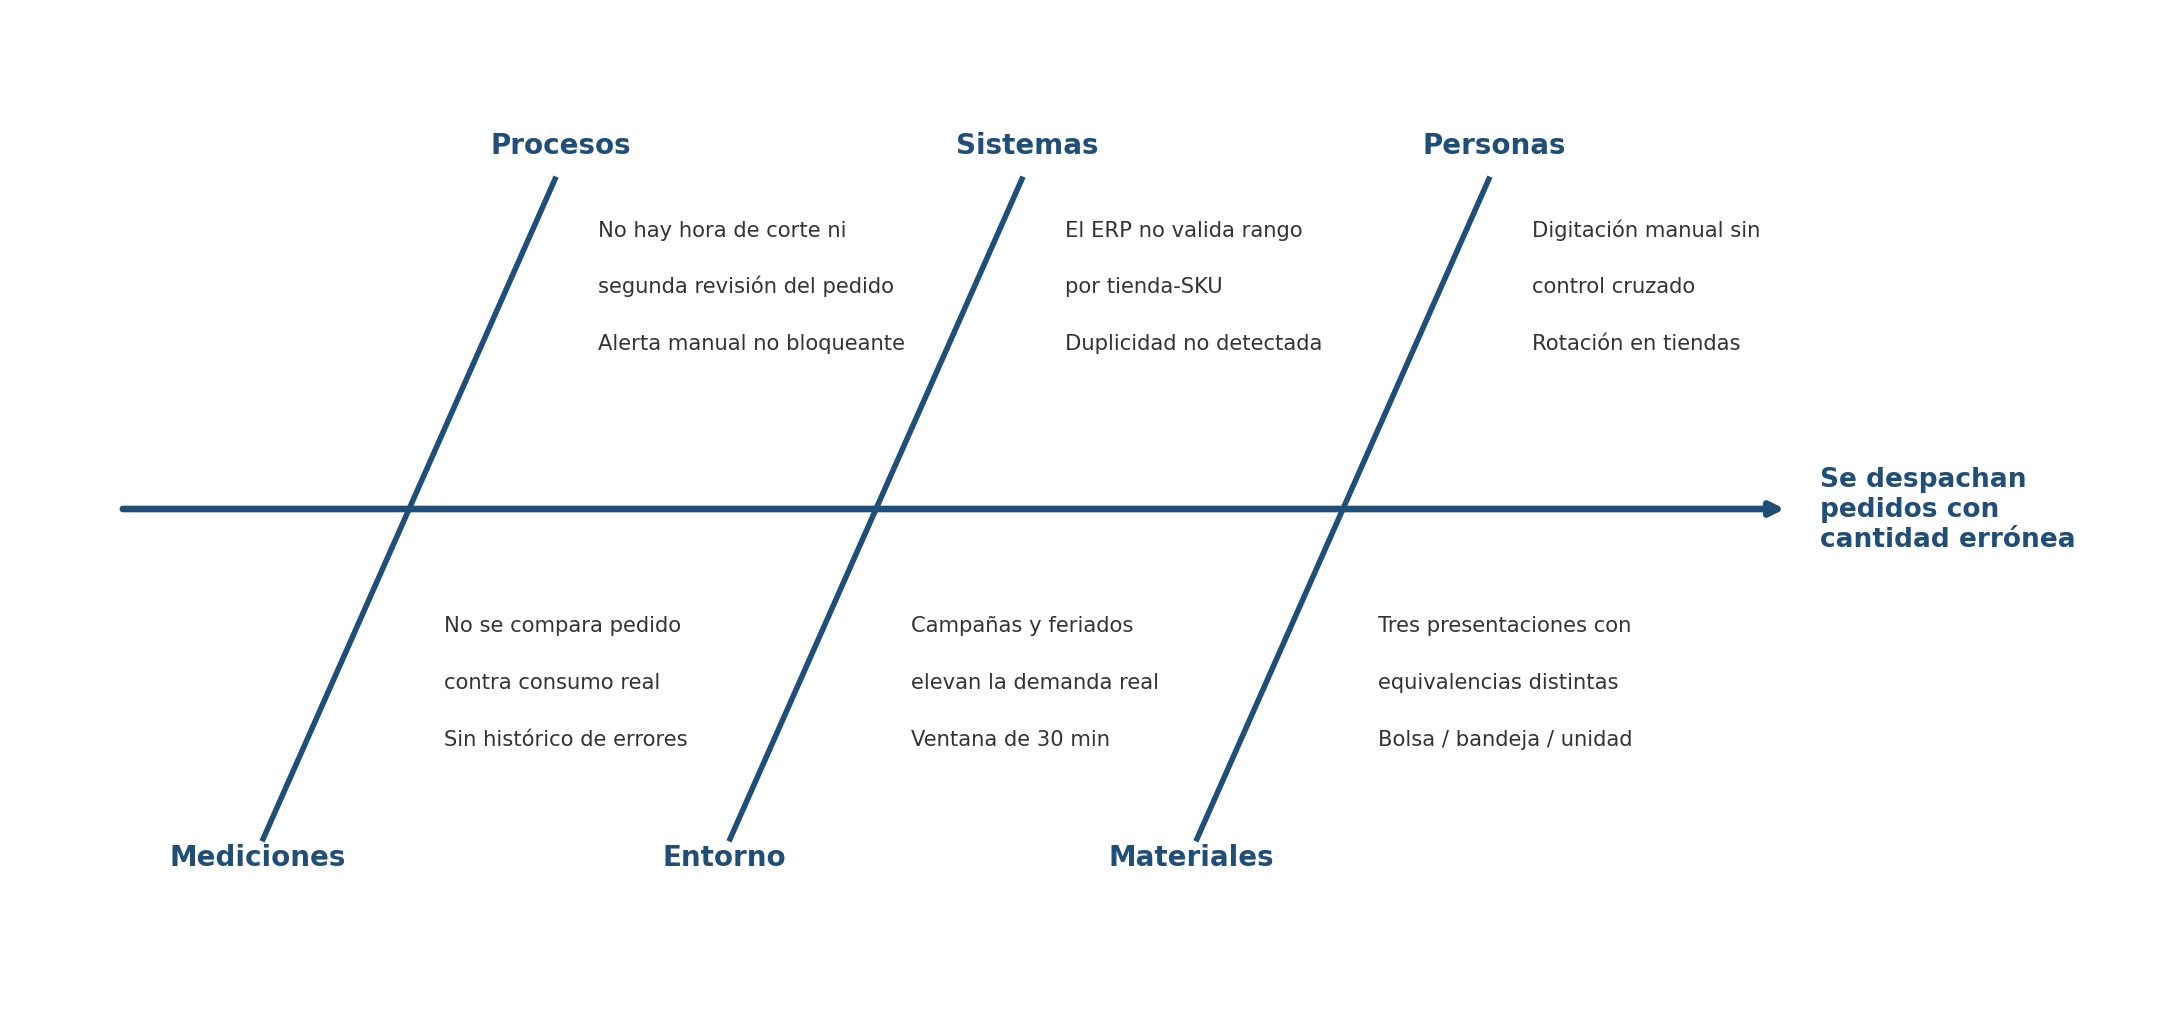
\includegraphics[width=\segun{}{0.75}\textwidth]{ishikawa.png}
\caption{Diagrama de causa--efecto sobre el despacho de pedidos con cantidad errónea \cite{ishikawa}. Las causas de Sistemas y Mediciones son las que este proyecto ataca; las de Entorno explican los falsos positivos que el modelo debe evitar.}
\label{fig:ishikawa}
\end{figure}

\subsection{La evidencia}

Tres correos de la operación sostienen lo anterior. El primero (Figura~\ref{fig:correo1}) es el mensaje interno que \segun{originó la revisión: advierte}{originó la revisión y advierte} cantidades altas en las tres presentaciones, con doble pedido en varias tiendas.

\iffinal\else
\begin{figure}[htbp]
\centering
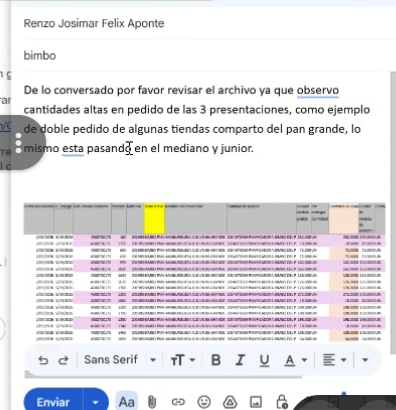
\includegraphics[width=0.5\textwidth]{correo_interno.png}
\caption{Comunicación interna que reporta cantidades altas y doble pedido en las tres presentaciones de pan de hamburguesa.}
\label{fig:correo1}
\end{figure}
\fi

Los otros dos muestran el control actual funcionando y fallando. En el segundo, el proveedor avisa que la tienda de ATE tiene un pedido «muy alto en comparación a su despacho anterior y el posterior» y recuerda que las alertas se responden en 30 minutos. \segun{Vale la pena detenerse en esa frase: el criterio que usa la analista es exactamente comparar contra el período anterior, que es lo que este proyecto quiere automatizar.}{El criterio que usa la analista es comparar contra el periodo anterior, que es lo que este proyecto busca automatizar.}

En el tercero, nadie contestó dentro de la ventana y el pedido se despachó igual, para no desabastecer la tienda. \segun{El control existe, pero no bloquea nada.}{Es decir, el control existe, pero no detiene el despacho.}

\iffinal
\begin{figure}[htbp]
\centering
\begin{minipage}[b]{0.31\textwidth}\centering
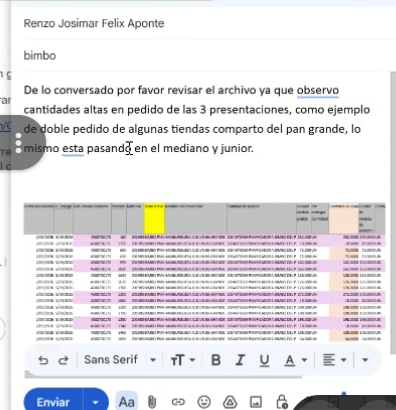
\includegraphics[width=\textwidth]{correo_interno.png}
\subcaption{Reporte interno de cantidades altas y doble pedido.}\label{fig:correo1}
\end{minipage}\hfill
\begin{minipage}[b]{0.33\textwidth}\centering
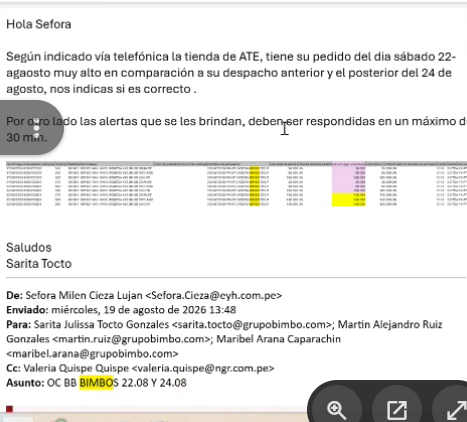
\includegraphics[width=\textwidth]{correo_alerta.png}
\subcaption{Alerta del proveedor sobre el pedido de ATE.}\label{fig:correo2}
\end{minipage}\hfill
\begin{minipage}[b]{0.33\textwidth}\centering
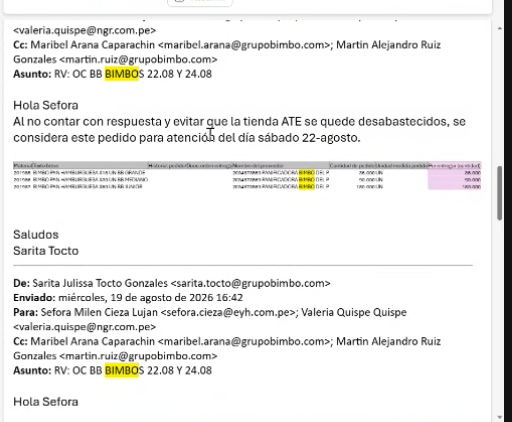
\includegraphics[width=\textwidth]{correo_sin_respuesta.png}
\subcaption{Sin respuesta, el pedido se atiende igual.}\label{fig:correo3}
\end{minipage}
\caption{Correos de la operación que sostienen el problema.}
\label{fig:correos}
\end{figure}
\else
\begin{figure}[htbp]
\centering
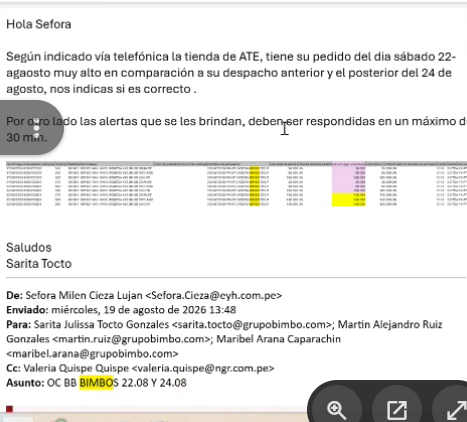
\includegraphics[width=0.55\textwidth]{correo_alerta.png}
\caption{Alerta manual del proveedor sobre el pedido atípico de una tienda, comparado contra el despacho anterior y el posterior.}
\label{fig:correo2}
\end{figure}

\begin{figure}[htbp]
\centering
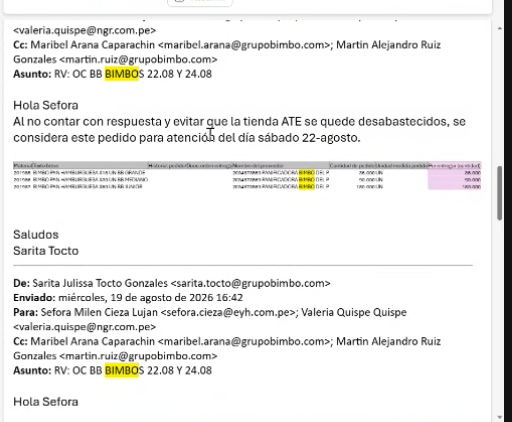
\includegraphics[width=0.6\textwidth]{correo_sin_respuesta.png}
\caption{Sin respuesta dentro de la ventana, el pedido sospechoso se atiende de todos modos.}
\label{fig:correo3}
\end{figure}
\fi

\subsection{El conjunto de datos}

El proyecto trabaja sobre un \segun{conjunto de datos real: el archivo}{conjunto de datos real, el archivo} \texttt{exportBIMBO.xlsx}, exportado del sistema de compras del cliente. Es la misma exportación que el área de planeamiento genera de forma rutinaria para revisar los pedidos, de modo que no hubo que construir nada para obtenerlo ni habrá que cambiar nada para volver a obtenerlo.

Cada fila del archivo es una \emph{línea de pedido}\segun{: }{, es decir, }un producto solicitado por una tienda para una fecha de entrega, dentro de una orden de compra. Una orden agrupa varias líneas, identificadas por su número de posición. El archivo tiene 10\,772 filas y 28 columnas, y cubre del 1 de julio al 11 de septiembre de 2026.

\iffinal\else
\begin{table}[htbp]
\centering
\caption{Muestra de las primeras filas del archivo.}
\label{tab:muestra}
\small
\begin{tabular}{@{}llrrlrr@{}}
\toprule
\textbf{Fe. entrega} & \textbf{Orden} & \textbf{Pos.} & \textbf{Material} & \textbf{Tienda} & \textbf{Cantidad} & \textbf{Valor S/} \\
\midrule
11-09-2026 & 4500730889 & 10 & 201985 & BB TDA MONTERRICO & 180 & 125,40 \\
11-09-2026 & 4500730889 & 20 & 201986 & BB TDA MONTERRICO & 330 & 193,60 \\
11-09-2026 & 4500730889 & 30 & 201987 & BB TDA MONTERRICO & 480 & 238,40 \\
11-09-2026 & 4500730889 & 40 & 201985 & BB TDA AURORA & 144 & 100,32 \\
11-09-2026 & 4500730889 & 50 & 201986 & BB TDA AURORA & 420 & 246,40 \\
11-09-2026 & 4500730889 & 60 & 201987 & BB TDA AURORA & 420 & 208,60 \\
\bottomrule
\end{tabular}
\end{table}
\fi

\subsubsection{Diccionario de columnas}

De las 28 columnas, 12 aportan información al análisis, 12 son constantes o administrativas y 4 vienen completamente vacías. \segun{La Tabla~\ref{tab:diccionario} las describe.}{Las columnas clave son la tienda, el material, la fecha de entrega y la cantidad pedida; las demás se usan como contexto, para el costo del exceso o como filtro.}

\iffinal\else
\begin{table}[htbp]
\centering
\caption{Columnas del archivo, su contenido y su uso en el proyecto.}
\label{tab:diccionario}
\small
\begin{tabularx}{\textwidth}{@{}L{4.2cm}Yc L{2.2cm}@{}}
\toprule
\textbf{Columna} & \textbf{Contenido} & \textbf{Valores distintos} & \textbf{Uso} \\
\midrule
Fecha documento & Día en que se registró la orden & 30 & Contexto \\
Fe. Entrega & Día comprometido de entrega & 68 & \textbf{Clave} \\
Documento compras & Número de orden de compra & 156 & Agrupación \\
Posición & Número de línea dentro de la orden & 197 & Duplicidad \\
Material & Código del producto & 3 & \textbf{Clave} \\
Texto breve & Descripción del producto & 3 & Reporte \\
Tienda & Nombre de la tienda solicitante & 61 & \textbf{Clave} \\
Centro & Código de la tienda & 61 & Equivale a Tienda \\
Cantidad de pedido & Unidades solicitadas & 115 & \textbf{Variable objetivo} \\
Cantidad en UMA & Igual a la anterior en este extracto & 115 & Verificación \\
Por entregar (cantidad) & Pendiente de despacho & 61 & Contexto \\
Valor neto de pedido & Importe de la línea en soles & 196 & Costo del exceso \\
Precio neto & Precio de referencia del producto & 59 & Contexto \\
Indicador de borrado & Marca «L» si la línea fue eliminada & 1 & \textbf{Filtro} \\
Creado por & Usuario que registró la orden & 23 & Contexto \\
Nombre del proveedor & Razón social del proveedor & 7 & Filtro \\
N.º Factura, Ref. Sunat, Fecha Pago & Datos de facturación, presentes en 6\,926 filas & -- & No se usan \\
Unidad medida pedido, Unidad de almacén, Moneda, Grupo de artículos, Cantidad base & Constantes en todo el archivo & 1 & No aportan \\
Historial pedido, Número de necesidad, Num. EM o AC, Tipo de imputación & Columnas vacías en las 10\,772 filas & 0 & No se usan \\
\bottomrule
\end{tabularx}
\end{table}
\fi


Tres observaciones sobre la calidad del archivo condicionan el análisis. La unidad de medida es única (UN) en todas las filas, de modo que no hay que convertir entre bolsas, bandejas y unidades dentro de este extracto. El campo de facturación está presente solo en 6\,926 filas, porque las órdenes más recientes aún no se facturan, así que no sirve para verificar lo entregado. Y el indicador de borrado obliga a un filtro previo que se explica en la Sección~\ref{sec:anuladas}.

Con los tres campos clave, que son tienda, material y fecha de entrega, más la cantidad, el archivo se reorganiza en 180 series semanales de tienda y producto, que son la materia prima del método. De ellas, 176 tienen suficiente historial previo para poder evaluarse, lo que deja 1\,554 observaciones de tienda, producto y semana sobre las que se mide todo lo que sigue.

\subsection{Qué dicen los datos}
\label{sec:datos}

Los correos describen el fenómeno; el extracto del sistema de compras permite medirlo. \segun{Conviene precisar el alcance de lo que sigue.}{Las cifras de esta sección tienen el siguiente alcance.} Las cifras y figuras de esta sección provienen de un análisis exploratorio \emph{ya ejecutado} sobre el extracto real, con un cuaderno en Python que se vuelve a correr sobre cualquier archivo del mismo formato. No son estimaciones ni ejemplos ilustrativos. Lo que todavía no existe es el software descrito en la Sección~\ref{sec:software}: el método está probado, la herramienta que lo pone en manos de quien revisa está por construirse. \segun{Los resultados de esta sección son, por tanto, la evidencia de que el enfoque funciona sobre los datos históricos, y no una medición del sistema en operación.}{Por tanto, estos resultados son un primer indicio de que el enfoque puede funcionar con los datos históricos; no son una medición del sistema en operación ni han sido validados en un periodo independiente (Sección~\ref{sec:av-periodos}).}

\subsubsection{Las líneas anuladas y el doble pedido}
\label{sec:anuladas}

Entre las columnas del archivo hay una llamada \emph{indicador de borrado}. Está vacía casi siempre, pero en 398 líneas dice «L», la marca que usa el sistema cuando una posición se elimina. \segun{Vale la pena mirarlas, porque cambian la cuenta.}{Estas líneas modifican los conteos, por lo que se analizaron por separado.}

De esas 398 líneas anuladas, 385 tienen al menos una línea activa para la misma tienda, el mismo producto y la misma fecha de entrega. \segun{No son pedidos adicionales: son pedidos}{No son pedidos adicionales, sino pedidos} que se borraron y se volvieron a cargar. Al comparar cada anulada con su reemplazo, en la enorme mayoría de los casos la cantidad es idéntica, es decir que se volvió a cargar exactamente lo mismo, y solo en 27 la cantidad cambió, con la versión definitiva mayor en 19 casos y menor en 8.

Esto obliga a trabajar con las 10\,374 líneas vigentes, y corrige una cuenta que sin ese filtro sale mal. Si se dejan las anuladas junto con sus reemplazos, el archivo aparenta tener cientos de pedidos repetidos con la misma cantidad, cuando en realidad se está contando dos veces el mismo pedido. Descontándolas quedan \textbf{54 casos de cantidad idéntica repetida}, que suman 119 líneas, y 176 combinaciones de tienda, producto y fecha con más de una línea. Ese es el volumen real del doble pedido, y para encontrarlo no hace falta \segun{ningún modelo: alcanza con}{ningún modelo, ya que alcanza con} una consulta.

\segun{Las 27 líneas donde la corrección cambió la cantidad sirven además como etiquetas: son pedidos que alguien registró de una forma y después rectificó.}{Las líneas donde la corrección cambió la cantidad (23 con el criterio de emparejamiento de la Sección~\ref{sec:av-limpieza}) son pedidos que alguien registró de una forma y después modificó. No se consideran errores por sí mismas, porque una modificación puede responder a una necesidad legítima de la tienda; se tratan como casos sospechosos que requieren evidencia (Sección~\ref{sec:av-marcado}).}

\subsubsection{El método encuentra el caso que ya conocíamos}

Se calculó, para cada tienda y producto, la mediana de las cuatro semanas previas como valor de referencia $\hat q_t$, y la diferencia relativa contra el pedido real, $e_t = (q_t - \hat q_t)/\hat q_t$. La Figura~\ref{fig:ate} muestra qué pasa con la tienda de ATE en pan grande.

Esa semana marcada es el pedido del sábado 22 de agosto, el mismo que motivó el correo de la Figura~\ref{fig:correo2}. El cálculo llegó a la misma conclusión que la analista, sin que nadie le indicara qué buscar. \segun{Es la mejor señal de que el criterio automático coincide con el juicio experto que hoy sostiene la verificación.}{Es un indicio de que el criterio automático puede coincidir con el juicio de la analista, aunque se basa en un solo caso confirmado.}

\begin{figure}[htbp]
\centering
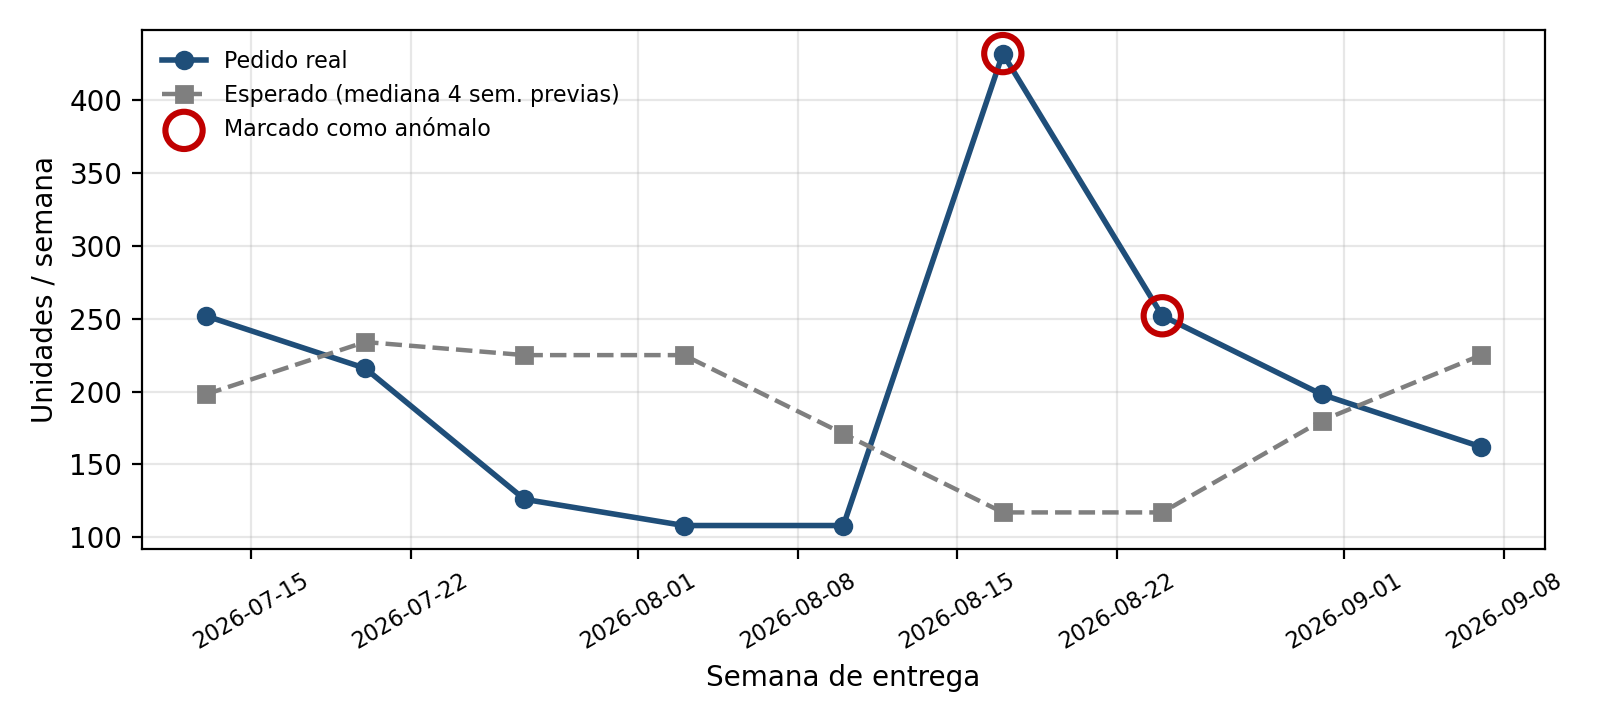
\includegraphics[width=\segun{0.9}{0.7}\textwidth]{ate_referencia.png}
\caption{\segun{Tienda ATE, pan grande: pedido real}{Tienda ATE, pan grande. Pedido real} contra valor de referencia. La semana del 17 de agosto pide 432 unidades donde se esperaban 117.}
\label{fig:ate}
\end{figure}

\subsubsection{Cuánto producto se despacha de más}

El impacto no está en la merma de la tienda sino en el \segun{propio despacho: se produce}{propio despacho, porque se produce}, se transporta y se factura una cantidad que el cliente no pidió realmente. Con el precio unitario implícito en cada línea (mediana S/~0,59) se puede poner número a ese exceso.

\begin{table}[htbp]
\centering
\caption{Exceso despachado sobre el valor de referencia, umbral $\tau = 0{,}8$.}
\label{tab:exceso}
\small
\begin{tabular}{@{}lr@{}}
\toprule
\segun{Casos detectados en 9 semanas evaluables}{Desviaciones detectadas en 9 semanas evaluables} & 17 \\
Exceso acumulado (unidades) & 11\,200 \\
Exceso acumulado (S/) & 6\,625 \\
\segun{\textbf{Exceso mensual estimado (S/)}}{\textbf{Valor potencial en riesgo al mes (S/)}} & \textbf{3\,187} \\
\bottomrule
\end{tabular}
\end{table}

\segun{Alrededor de \textbf{S/~3\,200 al mes} en producto despachado por encima de lo que el comportamiento del cliente permitía anticipar.}{Alrededor de \textbf{S/~3\,200 al mes} de \emph{valor potencial en riesgo}, es decir, el valor del producto que se habría despachado por encima de lo esperado si todas estas desviaciones fueran errores. No es una pérdida comprobada; la pérdida efectiva dependerá de cuántas desviaciones se confirmen como error (Sección~\ref{sec:av-terminos}).} La cifra descuenta el movimiento común de la cadena, según el procedimiento de la Sección~\ref{sec:campana}, y excluye las líneas anuladas.

\subsubsection{El feriado también levanta los pedidos}

No todas las alzas son errores. La semana del 27 de julio, Fiestas Patrias, llega al 12,4\,\% de series con alza superior al 50\,\%, frente a un nivel de fondo cercano al 2\,\%. Una regla de umbral marcaría veinte tiendas esa semana, todas correctas, y el analista dejaría de mirar las alertas en poco tiempo. Distinguir el feriado del error exige una pregunta que ningún umbral sobre una sola variable \segun{puede responder: si la tienda}{puede responder, la de saber si la tienda} subió sola o subió junto con todas las demás. La Sección~\ref{sec:campana} la responde con los datos.

\subsubsection{Separar la campaña del error sin preguntarle a nadie}
\label{sec:campana}

\segun{Un error de digitación de una tienda no mueve el promedio de las otras 175 series; un feriado sí.}{En el extracto, las 61 tiendas piden los mismos tres productos de pan de hamburguesa Bimbo (grande, mediano y junior), y cada combinación de tienda y producto forma una serie semanal. Por eso todas las series responden a la misma demanda de fondo. Cuando hay un feriado, suben muchas tiendas a la vez, mientras que un error de digitación afecta a una sola. Un error de una tienda no mueve el promedio de las otras 175 series; un feriado sí.} Sobre esa diferencia se puede construir un criterio que distinga ambos casos con los datos disponibles, sin depender de que alguien recuerde qué ocurrió una semana determinada.

Se define un \emph{factor común semanal} $a_t$ como la mediana del residuo de todas las series esa semana, y se descompone
\[
e_t \;=\; \underbrace{a_t}_{\text{lo que le pasó a todo el universo}} \;+\; \underbrace{u_t}_{\text{lo que le pasó solo a esta tienda}}.
\]
La decisión de anomalía se toma sobre $u_t$.

\begin{figure}[htbp]
\centering
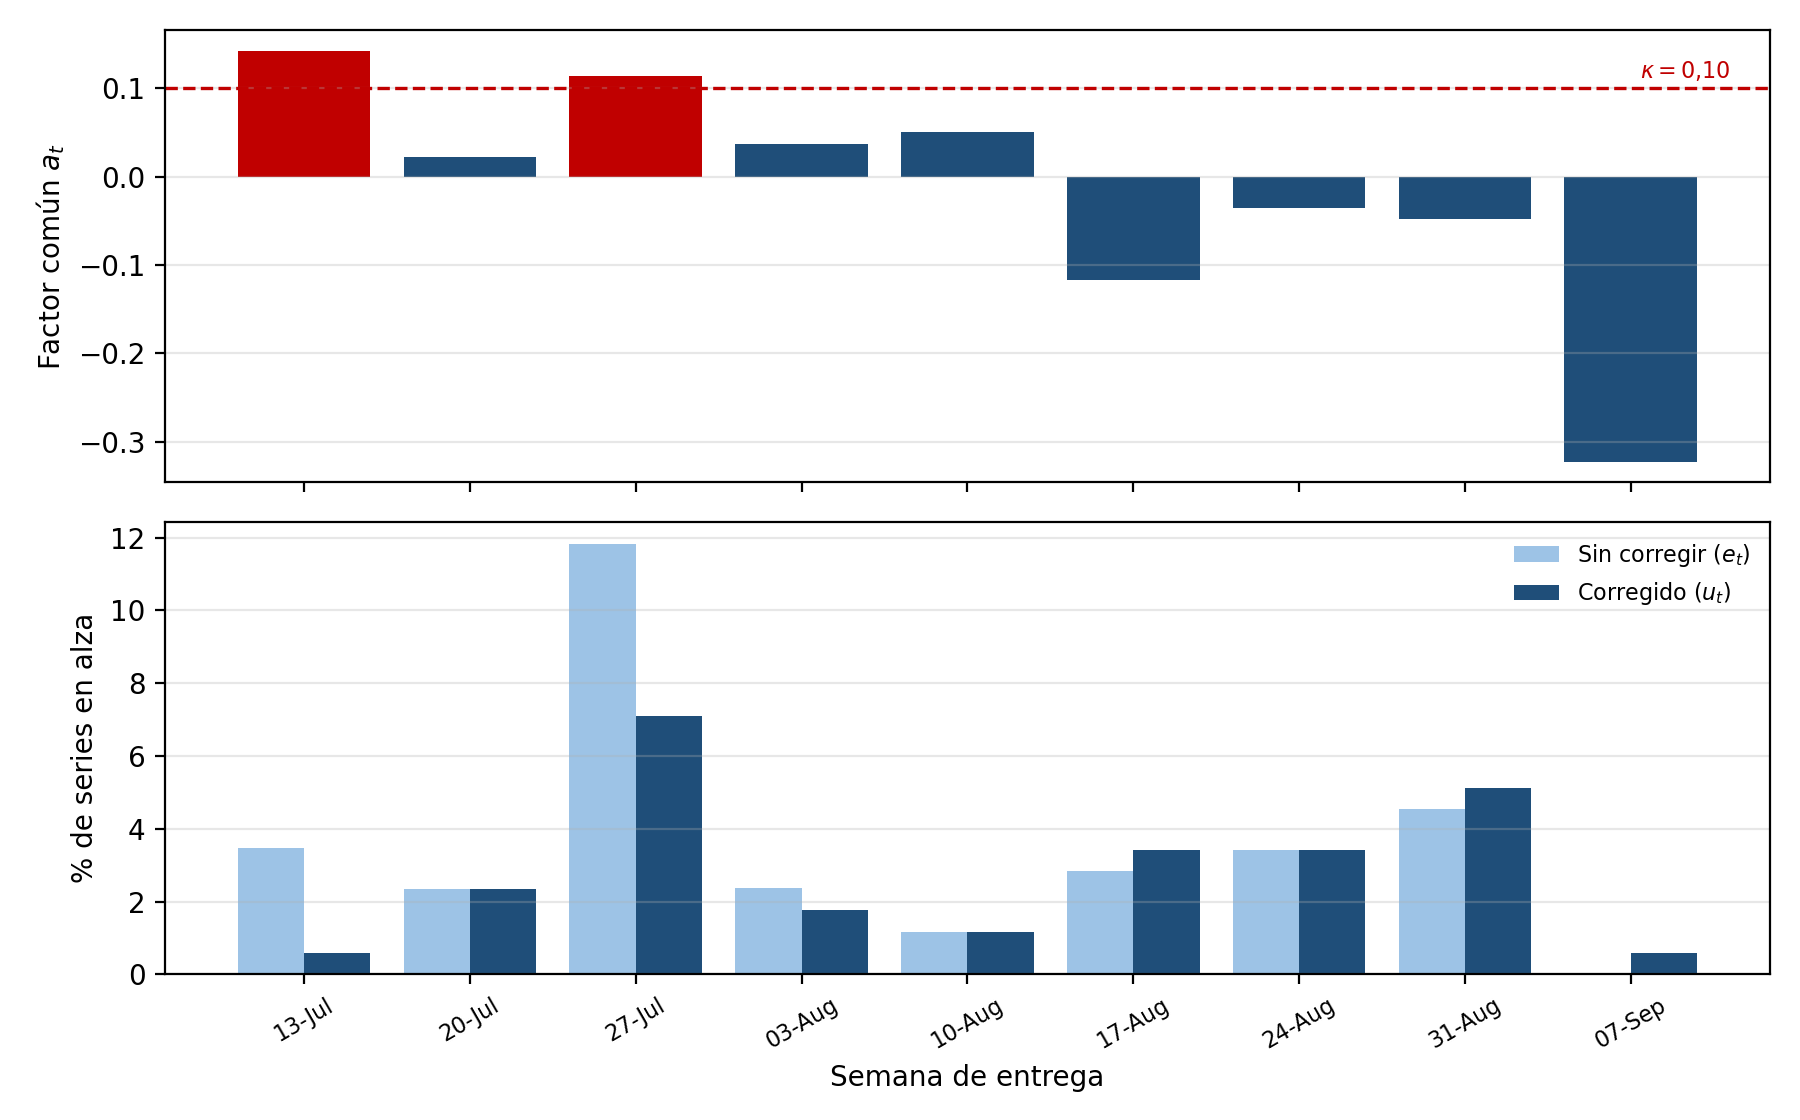
\includegraphics[width=\segun{0.9}{0.68}\textwidth]{factor_comun.png}
\caption{Arriba, el factor común semanal. Las dos semanas de julio que lo superan corresponden a movimientos de toda la cadena. Abajo, el porcentaje de series en alza antes y después de descontar ese factor.}
\label{fig:factor}
\end{figure}

La semana con mayor movimiento conjunto es la del 27 de julio, Fiestas Patrias, con un factor común de $+0{,}114$. Tres señales permiten separarla del caso de ATE, que es un error confirmado por correo.

\begin{table}[htbp]
\centering
\caption{Firma de una semana de campaña frente a la de un error de captura.}
\label{tab:firma}
\small
\begin{tabular}{@{}L{6cm}ll@{}}
\toprule
\textbf{Señal} & \textbf{27-jul (Fiestas Patrias)} & \textbf{17-ago (caso ATE)} \\
\midrule
Factor común $a_t$ & $+0{,}114$ & $-0{,}117$ \\
Series en alza, sin corregir & 12,4\,\% & 2,8\,\% \\
Series en alza, corregido & 7,7\,\% & 3,4\,\% \\
Tiendas que suben en las 3 presentaciones & 8 de 57 & 0 de 60 \\
Residuo mediano la semana siguiente & $+0{,}01$ & $+0{,}71$ \\
\bottomrule
\end{tabular}
\end{table}

\segun{Las dos últimas filas son las que más separan un caso del otro.}{Las dos últimas filas son las que más separan un caso del otro, pero la última usa información de la semana siguiente; por eso solo sirve para el análisis retrospectivo y no se usa para emitir alertas (Sección~\ref{sec:av-tiempo}).} En Fiestas Patrias suben las tres presentaciones a la vez en varias tiendas y el efecto se agota la semana siguiente, que vuelve a su nivel normal. En ATE ninguna tienda movió las tres presentaciones y el residuo sigue alto siete días después, que es el comportamiento esperable de un error arrastrado y no de un pico de consumo.

\subsubsection{Los parámetros del método}

El procedimiento no depende de un juicio externo, pero sí \segun{de cinco números que conviene nombrar y ajustar}{de cinco parámetros que deben ajustarse} con validación temporal en lugar de fijarlos a ojo.

\begin{table}[htbp]
\centering
\caption{Hiperparámetros del detector.}
\label{tab:hiper}
\small
\begin{tabularx}{\textwidth}{@{}cYcL{4cm}@{}}
\toprule
\textbf{Símbolo} & \textbf{Qué controla} & \textbf{Valor inicial} & \textbf{Cómo se ajusta} \\
\midrule
$k$ & Semanas de historial para la mediana de referencia & 4 & Error de predicción contra persistencia \\
$\tau$ & Cuánto tiene que desviarse una tienda por su cuenta ($u_t$) para marcar la línea & 0,8 & Precisión contra carga de alertas \\
$\kappa$ & Factor común a partir del cual la semana se declara de campaña & 0,10 & Semanas conocidas de feriado \\
$\sigma$ & Presentaciones que deben subir juntas para atenuar la alerta & 2 de 3 & Casos marcados como error \\
$\rho$ & Reversión esperada la semana siguiente para confirmar campaña & 0,00 & \segun{Histórico de semanas de feriado}{Solo análisis retrospectivo (usa la semana siguiente)} \\
\bottomrule
\end{tabularx}
\end{table}

Dejar la pregunta resuelta como parámetro y no como consulta tiene una \segun{ventaja sobre preguntar: el método}{ventaja sobre preguntar, ya que el método} vuelve a clasificar correctamente la próxima semana atípica sin que nadie tenga que recordar qué pasó en esta.

\subsubsection{Cuántas alertas serían}

\begin{figure}[htbp]
\centering
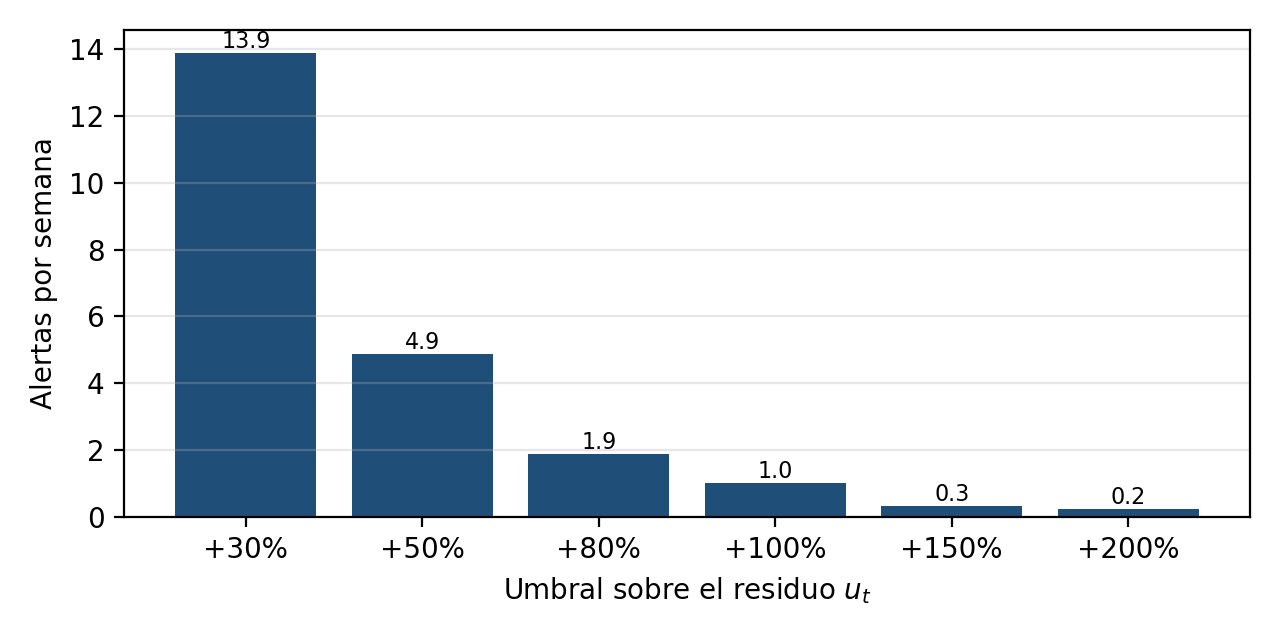
\includegraphics[width=\segun{0.85}{0.6}\textwidth]{alertas_umbral.png}
\caption{Alertas semanales esperadas según el umbral sobre $u_t$. Con $\tau = 0{,}8$ salen unas 2 por semana.}
\label{fig:alertas-umbral}
\end{figure}

Dos alertas por semana caben sin problema en la ventana de 30 minutos que ya está pactada. \segun{Un umbral más bajo detectaría más errores, pero a costa de un volumen que nadie va a revisar, y una alerta que no se revisa vale lo mismo que ninguna.}{Un umbral más bajo detectaría más errores, pero generaría más alertas de las que el área puede revisar.}

\subsection{A quién le duele}

\begin{table}[htbp]
\centering
\caption{Matriz impacto--interesados.}
\label{tab:impacto}
\small
\begin{tabularx}{\textwidth}{@{}L{2.6cm}YL{2.6cm}L{2.8cm}@{}}
\toprule
\textbf{Interesado} & \textbf{Cómo le afecta hoy} & \textbf{Magnitud al mes} & \textbf{Evidencia} \\
\midrule
Proveedor (Bimbo) & Produce, transporta y factura una cantidad distinta de la que el cliente realmente necesitaba & \segun{$\approx$ S/~3\,200}{$\approx$ S/~3\,200 en riesgo (potencial)} & Tabla~\ref{tab:exceso} \\
Planeamiento (Bimbo) & Revisa el archivo línea por línea y redacta los correos de confirmación & 17 casos por revisar cada 9 semanas & Figura~\ref{fig:correo2} \\
Compras (NGR) & Recibe la alerta, verifica con la tienda y rectifica la orden & \segun{27 líneas rectificadas en el extracto}{23 líneas modificadas en el extracto} & Indicador de borrado \\
Tiendas & Reciben una cantidad que no corresponde a su pedido & 54 casos de cantidad repetida & Sección~\ref{sec:anuladas} \\
Producción (Bimbo) & Planifica sobre una señal de demanda distorsionada & Indirecta & Efecto conocido en cadenas de suministro \cite{lee1997} \\
\bottomrule
\end{tabularx}
\end{table}

\subsection{Los stakeholders y quién decide}

\begin{table}[htbp]
\centering
\caption{Ubicación de los interesados según poder e interés.}
\label{tab:stakeholders}
\small
\begin{tabularx}{\textwidth}{@{}L{3.2cm}L{3.2cm}YL{2cm}@{}}
\toprule
\textbf{Interesado} & \textbf{Cuadrante} & \textbf{Qué necesita} & \textbf{Frecuencia} \\
\midrule
Jefatura de planeamiento (Bimbo) & Alto poder, alto interés & Que las alertas bajen su carga manual y sean defendibles ante el cliente & Semanal \\
Analista de planeamiento & Bajo poder formal, alto interés & Que el reporte llegue antes del cierre del pedido y no le sume trabajo & Semanal \\
Compras (NGR) & Alto poder, interés medio & Que la alerta no frene un pedido legítimo & Quincenal \\
Tiendas & Bajo poder, alto interés & No quedar desabastecidas por una alerta mal disparada & Por excepción \\
TI del cliente & Alto poder, bajo interés & Que nada de esto exija tocar el ERP en esta etapa & Por hito \\
\bottomrule
\end{tabularx}
\end{table}

\textbf{\segun{Responsable del resultado:}{Responsable del resultado,}} Sefora Cieza Lujan, autora del proyecto. Lo ejecuta \segun{de principio a fin: la preparación}{de principio a fin, incluida la preparación} de los datos, el marcado de los casos, el modelo y el software. La jefatura recibe el resultado al cierre y el asesor aprueba el entregable académico, pero ninguna etapa intermedia depende de que un tercero responda.

\iffinal\else
\begin{table}[htbp]
\centering
\caption{Responsabilidades sobre los entregables (RACI).}
\label{tab:raci}
\small
\begin{tabular}{@{}lcccc@{}}
\toprule
\textbf{Actividad} & \textbf{Practicante} & \textbf{Asesor} & \textbf{Jefatura} & \textbf{Cliente} \\
\midrule
Preparación y limpieza de datos & R/A & I & I & I \\
Marcado de los casos que fueron error & R/A & C & I & I \\
Construcción y validación del modelo & R/A & C & I & I \\
Calibración del umbral de alerta & R/A & C & I & I \\
Construcción del software & R/A & I & I & I \\
Presentación de resultados a la empresa & R & I & A & I \\
Aprobación del entregable académico & R & A & I & I \\
\bottomrule
\end{tabular}
\end{table}
\fi


\section{La solución}

\subsection{La propuesta}

La solución es un software de validación de pedidos. Quien revisa los pedidos carga el Excel que ya exporta del sistema de compras y el programa devuelve otro con los productos cuyo pedido no coincide con lo que el historial del cliente permitía esperar. \segun{Un archivo entra, un archivo sale, y en lugar de revisar miles de líneas una por una el analista revisa las pocas que quedan marcadas.}{En lugar de revisar miles de líneas una por una, el analista revisa solo las que quedan marcadas.} El programa \segun{no reemplaza la decisión: para cada}{no reemplaza la decisión, ya que para cada} producto marcado indica cuánto pidió la tienda, cuánto se esperaba según sus semanas anteriores y por qué se marcó, de modo que esa misma fila sirva para reclamarle al cliente. La confirmación final sigue siendo humana.

\segun{Hay dos caminos más obvios que este y ninguno funciona acá.}{Se consideraron otras dos opciones más directas, que se descartaron.} Un tope fijo de cantidad en el ERP trataría igual a una tienda de centro comercial que a una de barrio, y exigiría modificar un sistema que no controlamos. Pedir a las tiendas que confirmen cada pedido por segunda vez agrega un paso diario a un flujo que ya va apurado y \segun{no aprende nada: dentro de un año}{no aprende nada, y dentro de un año} el problema sigue igual. Calcular el valor esperado desde el propio historial evita ambos inconvenientes, porque cada tienda se compara consigo misma y el criterio mejora conforme se acumulan semanas. Es además lo que el área ya hace a mano cuando compara un pedido contra el despacho anterior, así que automatizarlo no le pide a nadie cambiar de forma de pensar.

Dentro de ese enfoque, el árbol de decisión \cite{breiman1984,quinlan1993} se eligió por una razón práctica antes que estadística. Para reclamarle a un cliente hace falta poder \segun{decirle por qué: según sus}{decirle por qué. Por ejemplo, según sus} últimas cuatro semanas esperábamos 117 unidades, usted pidió 432, y además hay una línea duplicada. \segun{Un modelo que solo entrega un puntaje traslada el problema de confianza en lugar de resolverlo.}{Un modelo que solo entrega un puntaje no permite dar esa explicación.}

La variable que no se mueve es la \textbf{precisión de las alertas}. Un sistema que marca de más se deja de mirar, que es el fracaso ya documentado en la Figura~\ref{fig:correo3}. Lo primero que cede es la \textbf{cobertura}\segun{: }{, ya que }se prefiere dejar pasar algunos errores pequeños antes que inundar de avisos al analista. También cede el \textbf{alcance de la integración}, porque el software trabaja sobre el archivo exportado y no toca el ERP del cliente.

\subsection{Por qué el proyecto se limita a estos datos}
\label{sec:limite}

El trabajo se restringe al pan de hamburguesa que Bimbo despacha a las tiendas Bembos \segun{operadas por NGR y EyH: tres productos}{operadas por NGR y EyH, con tres productos}, 61 tiendas y 11 semanas de historial. No se abordan otros proveedores, categorías ni cadenas.

\segun{La restricción es deliberada y mejora el resultado.}{Esta restricción se tomó por las siguientes razones.} Las tres presentaciones comparten unidad de medida, ciclo de reposición y comportamiento estacional, de modo que el valor esperado de una tienda es comparable con el de otra y el factor común semanal tiene sentido. Al ampliar a categorías con rotación distinta ese supuesto se rompe y habría que estimar un modelo por familia con menos datos cada uno. Trabajar sobre un universo cerrado permite además verificar \segun{contra hechos conocidos: el caso}{contra hechos conocidos, como el caso} de la tienda de ATE está documentado por correo y sirve de comprobación de que el método detecta lo que debe, contraste que no existiría en un conjunto disperso de proveedores. La generalización a otras categorías queda como continuación natural, una vez validado el método en este universo.

\subsection{Cómo funciona}

El sistema corre sobre el archivo de pedidos antes del despacho y tiene dos partes. La primera calcula, con el historial hasta la semana anterior, cuánto debería pedir cada tienda de cada producto. La segunda compara ese número con el pedido real y decide si la diferencia es normal, usando un árbol de decisión \cite{breiman1984,quinlan1993} sobre el residuo $e_t = (q_t - \hat q_t)/\max(\hat q_t, 1)$ y las variables de la Tabla~\ref{tab:variables}.

Para el valor esperado $\hat q_t$ se probarán tres opciones, de la más simple a la \segun{más elaborada: el pedido de la semana anterior}{más elaborada. La primera es el pedido de la semana anterior}, $\hat q_t = q_{t-1}$, que es lo que hace hoy la analista y por eso es la referencia obligada; la mediana de las cuatro semanas previas, que aguanta que el propio historial tenga pedidos equivocados, cosa que el promedio no hace; y suavizamiento exponencial con ajuste por día de la semana \cite{hyndman2021}, si el histórico da para tanto. Hay un detalle que puede arruinar el cálculo \segun{si se pasa por alto: el historial}{si se pasa por alto, y es que el historial} contiene los errores que se quieren detectar, así que la referencia sale inflada. Por eso se usan estimadores robustos y se recalcula excluyendo lo que la primera pasada marcó.

\subsection{Con qué variables decide el árbol}

\begin{table}[htbp]
\centering
\caption{Variables del clasificador.}
\label{tab:variables}
\small
\begin{tabularx}{\textwidth}{@{}lY@{}}
\toprule
\textbf{Variable} & \textbf{Qué mide} \\
\midrule
$e_t$ & Diferencia relativa entre lo pedido y lo esperado. \\
$z_{rob}$ & Cuántas desviaciones robustas se aleja el pedido de la mediana de su serie. \\
$\Delta_{prev}$ & Variación contra el pedido de la semana anterior. \\
$d_{dup}$ & Si existe otra línea con la misma tienda, producto y cantidad en la misma fecha. \\
$\rho_{mix}$ & Peso del producto dentro del pedido total de la tienda, comparado con su peso histórico. \\
$c_{sku}$ & Si las tres presentaciones se movieron juntas. Cuando suben todas a la vez suele ser demanda real. \\
$a_t$ & Mediana del residuo de todas las series esa semana. Separa el feriado del error de una tienda sola. \\
\textit{dow} & Día de la semana de entrega. \\
\bottomrule
\end{tabularx}
\end{table}

\segun{Las variables $c_{sku}$ y $a_t$ salen del hallazgo de la Sección~\ref{sec:campana} y son las que un umbral simple no puede usar.}{Las variables $c_{sku}$ y $a_t$ salen del hallazgo de la Sección~\ref{sec:campana} y son las que un umbral simple no puede usar. Todas se calculan solo con la información registrada hasta el momento de evaluar cada línea; ninguna usa datos de semanas posteriores (Tabla~\ref{tab:av-disponibilidad}).}

\subsection{De dónde sale la etiqueta}

El extracto no trae un campo que diga «este pedido estuvo mal», así que hay que construirlo en dos pasos. Primero se marcan como candidatos los casos que \segun{el área ya reconoce: duplicidad}{el área ya reconoce, como la duplicidad} exacta, residuo por encima del umbral acordado, diferencia entre lo pedido y lo consumido. Después se revisan uno por uno y se marcan como error o como normales.

\segun{Hay dos fuentes adicionales de etiquetas. Los correos de alerta guardan casos ya confirmados por escrito. Y de las 398 líneas anuladas, 27 fueron reemplazadas por una cantidad distinta: son pedidos que alguien registró de una forma y luego rectificó, es decir, errores reconocidos por la propia operación sin costo de revisión adicional.}{Un caso solo se considera \emph{error confirmado} cuando lo respalda evidencia operativa, como un correo de alerta en que el área o la tienda reconoce el error, una corrección del pedido acompañada de su motivo o la confirmación expresa de la analista. Las líneas anuladas y reemplazadas por otra cantidad no se cuentan como errores de forma automática, porque la modificación puede deberse a un cambio legítimo de necesidad (Sección~\ref{sec:av-marcado}).}

\subsection{Contra qué se compara}

El árbol se mide contra tres referencias. Un umbral sobre el pedido anterior, que reproduce el control manual actual y es el piso obligado; un umbral sobre $z_{rob}$, como regla estadística simple; y un Isolation Forest \cite{liu2008}, que no necesita etiquetas y sirve para verificar si el criterio de etiquetado tiene sentido. El árbol se implementa en \texttt{scikit-learn} con profundidad limitada \cite{pedregosa2011}, y se usa gradient boosting \cite{chen2016} solo como techo de referencia, para saber cuánta exactitud cuesta la interpretabilidad; si se usa, se acompaña de valores de Shapley \cite{lundberg2017}.

Si el árbol no le gana a los umbrales, \segun{hay que decirlo: que el problema}{hay que decirlo. Que el problema} se resuelva con una regla simple es un resultado válido, no un fracaso. El marco general de la tarea y sus métricas sigue a Chandola et al.\ \cite{chandola2009}, Hodge y Austin \cite{hodge2004} y Aggarwal \cite{aggarwal2017}; el proceso de trabajo sigue las fases de CRISP-DM \cite{wirth2000} dentro del marco del PMBOK \cite{pmbok2025} y la adaptación de la forma de trabajo de Ambler y Lines \cite{ambler2023}.

\subsection{El pedido que no llegó}
\label{sec:ausencias}

Un pedido con cantidad equivocada se ve en el archivo; uno que nunca se emitió, no. Para el proveedor la segunda situación \segun{puede costar más: la tienda}{puede costar más, porque la tienda} se queda sin producto, la venta no ocurre y nadie se entera hasta que alguien reclama.

El mismo cálculo que estima cuánto debería pedir una tienda detecta esos casos. Si una serie tienda--producto tiene valor esperado positivo para la semana en curso y en el archivo no aparece ninguna línea, la ausencia se reporta igual que una desviación de cantidad.

Las 180 series de tienda y producto por 11 semanas dan 1\,980 combinaciones posibles, de las cuales 1\,913 tienen pedido. Faltan 67, y \textbf{21 son huecos intermedios}\segun{: }{, es decir, }semanas sin pedido entre semanas con pedido, repartidos en 7 series de tres tiendas. No están dispersos en el tiempo, sino concentrados entre el 20 de julio y el 10 de agosto, y las tres tiendas dejan de pedir y vuelven en fechas próximas.

Ese patrón importa para el diseño. Una ausencia no es por sí sola \segun{un error: puede ser}{un error, ya que puede ser} una pausa con motivo, y varias tiendas que se detienen a la vez en la misma ventana apuntan a una causa compartida antes que a olvidos independientes. Distinguir una cosa de la otra exige el mismo contexto histórico que el resto del método y no un criterio aparte.

El software reporta las ausencias en una hoja separada del archivo de salida, con la tienda, el producto, la cantidad esperada y cuántas semanas lleva sin pedir, y deja la interpretación a quien conoce la operación.

\subsection{El software}
\label{sec:software}

El entregable final es un software de validación de pedidos que funciona de la forma más \segun{simple posible: }{simple posible, en la que }\textbf{\segun{entra un Excel y sale un Excel}{entra un Excel y sale otro}}. Quien revisa los pedidos carga el mismo archivo que hoy exporta del sistema de compras, sin transformaciones previas, y el programa devuelve otro con los productos cuyo pedido no coincide con lo que su historial permitía esperar. Lo que hoy significa recorrer miles de líneas a la vista pasa a ser revisar las pocas que quedan marcadas.

\segun{Entre esos dos extremos hay cuatro pantallas.}{La pantalla principal se describe a continuación; la arquitectura completa del software se presenta en la Sección~\ref{sec:arquitectura}.}

\iffinal\else
\subsubsection{Cargar el archivo}

\segun{El usuario arrastra el Excel}{El usuario selecciona el Excel} y el programa revisa que sirva antes de procesarlo: que estén las columnas necesarias, que las fechas sean fechas y las cantidades números, y que el archivo corresponda al proveedor esperado. Si algo falta, lo dice con nombre propio, «no encuentro la columna Fe.Entrega», en lugar de fallar sin explicación. También avisa cuántas líneas anuladas encontró y cuántas va a analizar, para que el usuario sepa sobre qué está trabajando.


\fi
\subsubsection{Revisar las alertas}

La pantalla principal es una tabla con una fila por producto marcado, ordenada por valor en riesgo, con las columnas de la Tabla~\ref{tab:columnas-salida} y filtros por tienda, producto y nivel de alerta.

\begin{table}[htbp]
\centering
\caption{Columnas del resultado.}
\label{tab:columnas-salida}
\small
\begin{tabularx}{\textwidth}{@{}L{4cm}Y@{}}
\toprule
\textbf{Columna} & \textbf{Contenido} \\
\midrule
Tienda & Nombre y código de la tienda. \\
Material y descripción & Código y texto breve del producto. \\
Fecha de entrega & Fecha comprometida de la línea. \\
Cantidad pedida / esperada & Lo solicitado y lo que el historial anticipaba. \\
Desviación & Diferencia porcentual entre ambas. \\
Motivo & Cantidad fuera de rango, duplicidad, o ambas. \\
Nivel & Alta, media o baja, según cuánto supere el umbral. \\
Valor en riesgo & Exceso en unidades por el precio unitario. \\
Últimas semanas & Pedidos previos de esa tienda y producto. \\
\bottomrule
\end{tabularx}
\end{table}

Al hacer clic en una fila se abre una \emph{ficha de detalle} con lo que el analista necesita para decidir \segun{sin salir del programa: el gráfico}{sin salir del programa, como el gráfico} de las últimas semanas de esa tienda y producto con el pedido actual resaltado, las otras dos presentaciones de la misma tienda esa semana, porque si subieron las tres es más probable que sea demanda real, y la regla exacta que disparó la alerta escrita en palabras.

Desde la misma ficha el analista marca la alerta como \emph{confirmada} o \emph{descartada}, y en el segundo caso escribe por qué. Ese registro de decisiones tiene un efecto que va \segun{más allá del orden: cada semana}{más allá del orden, ya que cada semana} de uso genera ejemplos etiquetados sin trabajo adicional, de modo que el modelo puede reentrenarse con casos reales en lugar de depender de una única muestra revisada al inicio. \segun{La herramienta produce, usándose, el insumo que necesita para mejorar.}{Así, el uso de la herramienta genera los datos necesarios para mejorarla.}

\iffinal\else
\subsubsection{Ver lo que no llegó}

Una segunda pestaña muestra las ausencias de pedido descritas en la Sección~\ref{sec:ausencias}: tiendas y productos que debían pedir esa semana y no aparecen en el archivo, con la cantidad esperada y cuántas semanas llevan sin pedir. En la cabecera aparece además el aviso de campaña cuando el movimiento común de la semana supera el umbral $\kappa$, para que nadie interprete como error un alza que afectó a toda la cadena.

\subsubsection{Exportar}

El botón de descarga genera el Excel de salida con las alertas, las ausencias y las decisiones tomadas. Es el archivo que se adjunta al correo del cliente, y reemplaza el que hoy se arma a mano.

Una pantalla de configuración permite ajustar el umbral de alerta y la ventana de historial sin tocar el código, porque esos valores se calibran con el uso y no deberían requerir a un programador cada vez.

\subsubsection{Cómo está construido}

Se construye en Python con \texttt{pandas} y \texttt{scikit-learn} \cite{pedregosa2011}, \segun{y la interfaz se arma con Streamlit, que convierte un script de análisis en una aplicación con carga de archivos, tablas, filtros y gráficos sin escribir código de frontend. Corre en el equipo del usuario.}{y la interfaz es una ventana de escritorio hecha con Tkinter, la librería gráfica incluida en Python. La ventana es la parte visible (\emph{front-end}) y el análisis con el árbol de decisión es la parte interna (\emph{back-end}), como se detalla en la Sección~\ref{sec:arquitectura}. Corre en la computadora de la usuaria.} \segun{Internamente encadena cinco pasos: lee y valida el archivo, agrupa por tienda--producto--semana, calcula el valor esperado con la mediana de las $k$ semanas previas, separa el movimiento común de la cadena del propio de cada tienda, y aplica el árbol entrenado devolviendo la marca junto con la regla que la produjo.}{Internamente encadena cinco pasos. Lee y valida el archivo, calcula para cada tienda y producto la referencia con las $k$ semanas previas, evalúa cada línea con lo registrado hasta su fecha de registro (Sección~\ref{sec:av-pedido}), separa el movimiento común de la cadena del propio de cada tienda y aplica el modelo elegido, que devuelve la marca junto con la regla que la produjo.} El modelo entrenado se guarda en disco, así que no reentrena en cada ejecución y responde en segundos. No requiere servidor, base de datos ni conexión con el ERP: trabaja sobre el archivo, igual que hoy trabaja la analista.


\fi
\subsection{Objetivo}

\textbf{General.} Construir y validar un sistema que estime el pedido esperado por tienda y producto a partir del historial, y que clasifique con un árbol de decisión las desviaciones frente al pedido real, \segun{alcanzando una precisión de al menos 70\,\% sobre los casos marcados como error, con no más de cinco alertas semanales, dentro de las 12 semanas del proyecto.}{usando solo la información disponible antes del despacho, y que alcance, en un periodo de prueba independiente, una precisión de al menos 70\,\% y una exhaustividad de al menos 80\,\% sobre errores confirmados con evidencia operativa, con entre 2 y 5 alertas por semana y al menos 3 días de anticipación respecto de la entrega, dentro de las 12 semanas del proyecto.}

\begin{table}[htbp]
\centering
\caption{\segun{El objetivo, letra por letra.}{El objetivo general en formato SMART (específico, medible, alcanzable, relevante y con plazo).}}
\label{tab:smart}
\small
\begin{tabularx}{\textwidth}{@{}cY@{}}
\toprule
\textbf{S} & Detectar pedidos anómalos por tienda y producto antes del despacho, con la regla que justifica cada alerta. \\
\textbf{M} & Precisión $\geq 70$\,\% y exhaustividad $\geq 80$\,\% \segun{sobre el conjunto de casos marcados; entre 2 y 5 alertas por semana.}{sobre errores confirmados; entre 2 y 5 alertas por semana; anticipación mediana de al menos 3 días (Tabla~\ref{tab:indicadores}).} \\
\textbf{A} & Los datos existen (11 semanas, 61 tiendas), las herramientas son de uso libre y el volumen corre en un equipo estándar. \\
\textbf{R} & \segun{Ataca un costo de alrededor de S/~3\,200 al mes y una tarea manual que hoy no escala.}{Atiende un valor potencial en riesgo de alrededor de S/~3\,200 al mes y una tarea manual que hoy no escala.} \\
\textbf{T} & \segun{Semana 12 del proyecto, con validación temporal sobre las últimas tres semanas del extracto.}{Semana 12 del proyecto, evaluando una sola vez sobre las dos últimas semanas completas del extracto (24 y 31 de agosto), reservadas como prueba, y confirmando con un extracto posterior al 11 de septiembre.} \\
\bottomrule
\end{tabularx}
\end{table}

\iffinal
\subsection{Objetivos específicos}

Cada objetivo específico tiene un indicador y una fecha que permiten verificar su cumplimiento.

\begin{table}[htbp]
\centering
\caption{Objetivos específicos con su indicador de cumplimiento.}
\label{tab:obj-especificos}
\small
\begin{tabularx}{\textwidth}{@{}cYL{4.6cm}c@{}}
\toprule
\# & \textbf{Objetivo específico} & \textbf{Indicador y meta} & \textbf{Semana} \\
\midrule
1 & Limpiar y consolidar el extracto en una tabla tienda--producto--semana & El programa reproduce las cifras de la Sección~\ref{sec:datos} y excluye el 100\,\% de las líneas anuladas & 2 \\
2 & Calcular el valor esperado de cada línea con la información disponible al registrarla & Error medio de la referencia menor que el de usar la semana anterior & 7 \\
3 & Reunir casos de error confirmados con evidencia operativa & Al menos 20 errores confirmados, cada uno con su fuente & 7 \\
4 & Entrenar el árbol y las reglas sencillas y elegir el método con el periodo de validación & Decisión documentada en el hito H3 & 8 \\
5 & Construir el software que recibe el Excel y devuelve las líneas a revisar con su motivo & Resultado en menos de 60 segundos y cumplimiento de los 9 criterios de la Tabla~\ref{tab:aceptacion} & 11 \\
6 & Evaluar el método una sola vez en el periodo independiente & Precisión, exhaustividad, alertas por semana y anticipación reportadas frente a sus metas & 12 \\
\bottomrule
\end{tabularx}
\end{table}
\else
\subsection{Objetivos específicos}

\begin{enumerate}
\item Limpiar y consolidar el extracto en una tabla tienda--producto--semana.
\item Implementar el cálculo del valor esperado y compararlo contra la persistencia.
\item Marcar los casos que fueron error a partir del historial disponible.
\item Entrenar el árbol y las líneas base, y evaluarlos con validación temporal.
\item Construir el software que recibe el Excel de pedidos y devuelve los productos anómalos con su descripción, la desviación y el motivo.
\end{enumerate}
\fi

\section{Alcance y verificación}

\subsection{Qué entra y qué no}

\begin{table}[htbp]
\centering
\caption{Frontera del proyecto.}
\label{tab:frontera}
\small
\begin{tabularx}{\textwidth}{@{}YY@{}}
\toprule
\textbf{Dentro} & \textbf{Fuera} \\
\midrule
Limpieza y consolidación del extracto & Pronóstico de demanda para planificar producción \\
Cálculo del pedido esperado por tienda y producto & Integración dentro del ERP del cliente \\
Variables de desviación y contexto & Optimización de rutas, inventario o producción \\
Marcado de los casos que fueron error & Corrección automática del pedido \\
Árbol de decisión y líneas base, con validación temporal & Otros proveedores, otras categorías y otras cadenas (Sección~\ref{sec:limite}) \\
Software que recibe el Excel y devuelve los productos anómalos & Despliegue en producción y soporte posterior \\
\bottomrule
\end{tabularx}
\end{table}

La corrección automática del pedido queda fuera \segun{de manera deliberada: decidir}{de manera deliberada, porque decidir} por la tienda cuánto debe pedir excede la responsabilidad que el proyecto puede asumir en esta etapa.

\subsection{Restricciones, supuestos e incertidumbres}

\begin{table}[htbp]
\centering
\caption{Lo que se planifica, lo que se valida y lo que se investiga.}
\label{tab:rsi}
\small
\begin{tabularx}{\textwidth}{@{}YYY@{}}
\toprule
\textbf{Restricción} & \textbf{Supuesto} & \textbf{Incertidumbre} \\
\midrule
El extracto cubre 11 semanas y no se puede alargar hacia atrás & Que las cantidades son comparables entre líneas del mismo producto & Cuánta de la desviación de una semana de campaña es demanda y cuánta error \\
No se puede modificar el ERP del cliente & Que el historial de correos alcanza para marcar suficientes casos & \segun{Cuántos de los 27 pedidos rectificados}{Cuántos de los 23 pedidos modificados} son errores y cuántos cambios de necesidad \\
El proyecto cierra en la semana 12 & Que el extracto refleja operación normal y no un período atípico & Con qué frecuencia aparecen errores por debajo del umbral, que hoy no se detectan \\
Los datos deben anonimizarse para uso académico & Que las alertas se responden dentro de los 30 minutos pactados & Si el patrón se sostiene al ampliar el historial más allá de 11 semanas \\
\bottomrule
\end{tabularx}
\end{table}

\segun{El caso más peligroso no es que el sistema deje pasar un error, sino el contrario: que marque un pedido correcto, alguien le crea y recorte una cantidad que la tienda sí necesitaba.}{El riesgo de mayor impacto es que el sistema marque como error un pedido correcto y, por esa alerta, se recorte una cantidad que la tienda sí necesitaba.} Ahí el proyecto deja de ahorrar y empieza a costar, porque un quiebre de stock vale más que el exceso que se \segun{buscaba evitar: la venta}{buscaba evitar, ya que la venta} no ocurre y el reclamo pasa a ser del cliente hacia el proveedor. Los correos revisados muestran que la operación ya conoce ese riesgo y decide \segun{en su favor: ante la duda}{en su favor, porque ante la duda} se despacha igual, para no desabastecer.

De ahí salen dos decisiones de diseño que aparecen en todo el documento. El sistema alerta pero no bloquea, de modo que ninguna alerta puede reducir un pedido por sí sola. Y la precisión se prioriza sobre la cobertura, aceptando que se escapen errores pequeños antes que marcar pedidos legítimos.

\iffinal\else
\subsection{Qué se va a medir}

\begin{table}[htbp]
\centering
\caption{Evidencia mínima del proyecto.}
\label{tab:evidencia}
\small
\begin{tabularx}{\textwidth}{@{}L{3.6cm}YYl@{}}
\toprule
\textbf{Qué mido} & \textbf{Hoy} & \textbf{Con la solución} & \textbf{Cuándo} \\
\midrule
Pedidos erróneos detectados antes del despacho & Solo los que alguien nota al revisar el archivo & $\geq 80$\,\% de los confirmados & \segun{Semana 7}{Semana 12} \\
Precisión de las alertas & Sin medir & $\geq 70$\,\% & \segun{Semana 7}{Semana 12} \\
Alertas emitidas por semana & 1 documentada en el extracto & entre 2 y 5 & Semana 8 \\
Unidades despachadas de más y detectadas & 0 & $\geq 80$\,\% de las 11\,200 \segun{identificadas en el extracto}{unidades de desviación identificadas en el extracto} & Semana 12 \\
Tiempo entre la carga del archivo y el resultado & Revisión manual de todo el archivo & Menos de un minuto & Semana 10 \\
\bottomrule
\end{tabularx}
\end{table}

\subsection{Indicadores}

\begin{table}[htbp]
\centering
\caption{Indicadores de seguimiento.}
\label{tab:indicadores}
\small
\begin{tabularx}{\textwidth}{@{}L{2.6cm}YL{1.6cm}L{1.6cm}L{2.2cm}@{}}
\toprule
\textbf{Indicador} & \textbf{Cómo se calcula} & \textbf{Meta} & \textbf{Frecuencia} & \textbf{Fuente} \\
\midrule
Precisión & Alertas confirmadas como error / alertas emitidas & $\geq 70$\,\% & Semanal & Registro de casos marcados \\
Exhaustividad & Errores detectados / errores confirmados & $\geq 80$\,\% & Semanal & Registro de casos marcados \\
Carga de alertas & Alertas emitidas por semana & 2 a 5 & Semanal & Salida del software \\
Error del valor esperado & Error absoluto medio frente a la persistencia & $< 1$ & Semanal & Extracto \\
Unidades marcadas & Exceso en unidades sobre el valor esperado & Seguimiento & Semanal & Salida del software \\
\bottomrule
\end{tabularx}
\end{table}

\fi
\subsection{Criterios de aceptación del prototipo}

Cada criterio está redactado de modo que la respuesta sea verdadero o falso, sin lugar a interpretación, e indica quién lo verifica y con qué evidencia queda demostrado.

\begin{longtable}{@{}c p{8.6cm} L{2cm} L{3.2cm}@{}}
\caption{Criterios de aceptación del software.}\label{tab:aceptacion}\\
\toprule
\# & \textbf{Criterio} & \textbf{Quién verifica} & \textbf{Evidencia} \\
\midrule
\endfirsthead
\toprule
\# & \textbf{Criterio} & \textbf{Quién verifica} & \textbf{Evidencia} \\
\midrule
\endhead
\small 1 & \small Dado el archivo exportado del sistema de compras sin modificar, cuando se ejecuta la validación, entonces el software termina sin error y devuelve un Excel con las nueve columnas de la Tabla~\ref{tab:columnas-salida} completas en todas las filas. & \small Practicante & \small Archivo de salida de una semana real \\
\small 2 & \small Dado el caso documentado de la tienda de ATE en la semana del 17 de agosto, cuando se ejecuta la validación sobre ese período, entonces esa línea aparece marcada con nivel alto. & \small Practicante & \small Salida del software y correo de alerta original \\
\small 3 & \small Dadas dos líneas vigentes con la misma tienda, producto, fecha de entrega y cantidad, cuando se ejecuta la validación, entonces ambas quedan marcadas con motivo duplicidad. & \small Practicante & \small Salida sobre los 54 casos identificados en el extracto \\
\small 4 & \small Dada una serie tienda--producto con menos de $k$ semanas de historial, cuando se evalúa su pedido, entonces aparece en la hoja de no evaluables y no en la de anomalías. & \small Practicante & \small Salida del software \\
\small 5 & \small Dada una semana cuyo factor común supera $\kappa$, cuando se ejecuta la validación, entonces el reporte incluye la advertencia de posible campaña. & \small Practicante & \small Salida sobre la semana del 27 de julio \\
\small 6 & \small Dada una tienda con valor esperado positivo y sin ninguna línea en el archivo, cuando se ejecuta la validación, entonces aparece en la hoja de ausencias con las semanas que lleva sin pedir. & \small Practicante & \small Salida sobre las 7 series con huecos intermedios \\
\small 7 & \small Dado el mismo archivo de entrada, cuando se ejecuta la validación dos veces, entonces ambos resultados son idénticos. & \small Practicante & \small Comparación de los dos archivos de salida \\
\small 8 & \small Dado un archivo al que le falta una columna obligatoria, cuando se ejecuta la validación, entonces el software nombra la columna faltante y no procesa. & \small Practicante & \small Captura del mensaje de error \\
\small 9 & \small Dado el archivo de una semana, cuando lo ejecuta alguien ajeno al proyecto sin acompañamiento, entonces obtiene el resultado en menos de un minuto y sin consultar el manual. & \small Practicante & \small Acta de la prueba de uso \\
\bottomrule
\end{longtable}

\segun{El criterio 9 es el que suele darse por supuesto y no se escribe. Un software que entrega el resultado correcto pero que solo sabe ejecutar quien lo programó no resuelve el problema de nadie más.}{El criterio 9 busca asegurar que el software pueda ser usado por el área sin depender de quien lo programó.}

\subsection{Viabilidad}

\textbf{Técnica.} El volumen es pequeño y los modelos son ligeros. Python, \texttt{pandas} y \texttt{scikit-learn} bastan en un equipo corriente \cite{pedregosa2011}. El proyecto está dimensionado para el perfil de quien lo ejecuta, una ingeniera industrial con manejo de \segun{análisis de datos: no requiere}{análisis de datos, por lo que no requiere} desarrollo web, base de datos ni despliegue en servidores. \segun{La interfaz se arma con Streamlit, que convierte un script de análisis en una aplicación con carga de archivos, tablas y gráficos sin escribir código de frontend, y las reglas}{La interfaz es una ventana sencilla en Tkinter, incluida en Python, y las reglas} legibles del árbol se obtienen directamente de \texttt{export\_text} en \texttt{scikit-learn}. La parte propiamente informática del trabajo se reduce así a encadenar herramientas existentes.

\textbf{Operativa.} El área ya hace esta verificación a mano y aplica el mismo criterio de comparar contra el período anterior, así que el sistema no le pide cambiar de forma de pensar. Dos a cinco alertas semanales caben en la rutina que ya existe y en la ventana de 30 minutos ya pactada.

\segun{\textbf{Económica.} No hay licencias ni infraestructura que comprar. El costo es el tiempo de trabajo de la practicante. El exceso que hoy se despacha, unos S/~3\,200 al mes, supera el costo de las horas de validación necesarias para poner el sistema en marcha.}{\textbf{Económica.} No hay licencias ni infraestructura que comprar. El costo es, principalmente, el tiempo de las personas que participan, estimado en S/~3\,312 con reservas (Sección~\ref{sec:presupuesto}). El valor potencial en riesgo, del orden de S/~3\,200 al mes, es comparable a ese costo, aunque no constituye un ahorro comprobado.}

\iffinal\else
\subsection{Matriz de riesgos}

Cada riesgo lleva su probabilidad, su impacto y una \emph{señal temprana}: el dato observable que avisa que el riesgo se está materializando, antes de que sea tarde para reaccionar.

\begin{longtable}{@{}L{3.3cm}ccL{3.6cm}L{4.4cm}@{}}
\caption{Riesgos del proyecto.}\label{tab:riesgos}\\
\toprule
\textbf{Riesgo} & \textbf{Prob.} & \textbf{Imp.} & \textbf{Señal temprana} & \textbf{Mitigación} \\
\midrule
\endfirsthead
\toprule
\textbf{Riesgo} & \textbf{Prob.} & \textbf{Imp.} & \textbf{Señal temprana} & \textbf{Mitigación} \\
\midrule
\endhead
\small No se logran marcar suficientes casos como error & \small Alta & \small Alto & \small Al revisar los veinte candidatos, la mayoría queda en duda & \small Revisarlos en la semana 4; si no alcanzan, pasar a detección no supervisada y replantear las metas \\
\small Sobreajuste del árbol con 176 series y 3 productos & \small Media & \small Alto & \small La precisión en validación cae respecto de la de entrenamiento & \small Profundidad limitada, validación temporal, agrupar por presentación \\
\small La referencia queda inflada porque el historial contiene los errores & \small Alta & \small Medio & \small El valor esperado sube semana a semana sin que suba el consumo & \small Mediana y MAD en lugar de promedio; recálculo excluyendo lo marcado \\
\small Campañas y feriados generan alertas correctas pero inútiles & \small Media & \small Alto & \small Más del 10\,\% del universo supera el umbral la misma semana & \small Separar el movimiento de toda la cadena del de cada tienda (Sección~\ref{sec:campana}) \\
\small Muy pocos casos anómalos frente al total & \small Alta & \small Medio & \small La exactitud global supera el 95\,\% sin detectar nada & \small Reportar precisión y exhaustividad, nunca exactitud \\
\small El software no se adopta y se vuelve a la revisión manual & \small Media & \small Alto & \small En la prueba de la semana 12 alguien ajeno al proyecto no logra ejecutarlo solo & \small Criterio de aceptación 9; interfaz de un solo paso; formato de salida igual al que ya usan \\
\small Cambio en el formato del archivo exportado & \small Baja & \small Alto & \small Aparecen columnas nuevas o renombradas en el extracto & \small Verificación de columnas al inicio del proceso, con mensaje explícito \\
\small Pérdida de acceso a los datos & \small Baja & \small Alto & \small Demora en la entrega del extracto mensual & \small Copia anonimizada congelada al inicio del proyecto \\
\bottomrule
\end{longtable}

Los dos primeros riesgos son los que pueden cambiar el resultado del proyecto y no solo retrasarlo. El resto se administra dentro del plan.

\fi
\iffinal\else
\subsection{Plan de trabajo}
\label{sec:plan}

El proyecto lo ejecuta una sola persona de principio a fin. No hay un equipo ni un área que valide entregas intermedias: el resultado se presenta a la jefatura al cierre y a la universidad como entregable académico. El plan está armado en consecuencia, sin pasos que dependan de que responda un tercero.

Las dos primeras semanas ya están hechas. El análisis exploratorio de la Sección~\ref{sec:datos} cubre la limpieza del extracto, el cálculo del valor esperado, la separación del residuo, la detección de duplicados y de ausencias y la estimación del exceso, y funciona sobre los datos reales. Lo pendiente empieza en la semana 3.

\segun{Dos decisiones de orden vale la pena explicar.}{Sobre el orden de los pasos se tomaron dos decisiones.} Las reglas simples se miden antes de entrenar el árbol, no después, para que la comparación no se acomode al resultado: el número contra el que hay que ganar ya está escrito cuando el árbol se entrena. Y el paso 3 va antes que el 4 porque sin casos marcados no hay con qué medir ninguno de los dos.

El paso 10 merece una nota, porque es el que hace que la herramienta mejore con el uso. Cada vez que alguien confirma o descarta una alerta desde la ficha queda un ejemplo marcado, sin trabajo adicional. A las pocas semanas de operación hay más casos revisados que los del paso 3, y el modelo puede reentrenarse con ellos. El etiquetado deja de ser un esfuerzo puntual del inicio y pasa a ser un subproducto del uso.

El hito del paso 5 es el que puede cambiar el rumbo. Si el árbol no le gana a las reglas simples, se deja el árbol y el software se construye igual sobre la regla que haya ganado: cambia cómo se decide qué marcar, no el resto de la herramienta. Que el problema se resuelva con una regla sencilla es un resultado válido y así se reportaría.

\begin{longtable}{@{}c p{6.4cm} L{3.6cm} c L{1.8cm}@{}}
\caption{Pasos del proyecto, su producto, la semana en que cierran y la herramienta con que se hacen.}\label{tab:pasos}\\
\toprule
\# & \textbf{Paso} & \textbf{Qué queda al terminarlo} & \textbf{Sem.} & \textbf{Con qué} \\
\midrule
\endfirsthead
\toprule
\# & \textbf{Paso} & \textbf{Qué queda al terminarlo} & \textbf{Sem.} & \textbf{Con qué} \\
\midrule
\endhead
\multicolumn{5}{@{}l}{\textit{Hecho}} \\
\small 1 & \small \textbf{Limpiar el dataset y explorarlo.} Quitar las líneas anuladas, revisar formatos, armar las series semanales y medir el problema & \small Archivo limpio, el programa que lo limpia y las cifras de la Sección~\ref{sec:datos} & \small 1--2 & \small\texttt{pandas} \\
\midrule
\multicolumn{5}{@{}l}{\textit{Modelo}} \\
\small 2 & \small \textbf{Armar la tabla de señales.} Para cada pedido, calcular las ocho señales que después mirará el modelo & \small Tabla con una fila por pedido y sus ocho señales & \small 3--4 & \small\texttt{pandas} \\
\small 3 & \small \textbf{Marcar los casos que fueron error.} Revisar los candidatos uno por uno apoyándose en el historial de correos de alerta \segun{y en las 27 líneas que alguien rectificó}{y exigiendo evidencia operativa para cada error} & \small Lista de casos marcados como error o como normales & \small \segun{4--5}{4--7} & \small Excel \\
\small 4 & \small \textbf{Probar primero las reglas simples.} Medir tres métodos sencillos para saber contra qué hay que ganarle & \small Resultado de las tres reglas & \small 5--6 & \small\texttt{pandas}, \texttt{sklearn} \\
\small 5 & \small \textbf{Entrenar el árbol y compararlo} con las reglas del paso 4 & \small Comparación semana por semana. \textbf{Hito: se decide si el árbol se justifica} & \small \segun{6--7}{7--8} & \small\texttt{sklearn} \\
\small 6 & \small \textbf{Decidir a partir de cuánto se avisa}, buscando el punto donde el número de alertas por semana sigue siendo revisable & \small Umbral fijado y curva umbral--alertas & \small 8 & \small\texttt{pandas} \\
\small 7 & \small \textbf{Escribir el motivo en palabras.} Convertir lo que decide el modelo en una frase que el cliente entienda & \small Texto del motivo para cada alerta & \small 8 & \small\texttt{export\_text} \\
\midrule
\multicolumn{5}{@{}l}{\textit{Software}} \\
\small 8 & \small \textbf{Motor de cálculo.} Una función que recibe la ruta del Excel y devuelve la tabla de alertas & \small Programa que ya funciona, aunque sin pantallas & \small 9 & \small\texttt{pandas} \\
\small 9 & \small \textbf{Pantalla de carga y tabla de alertas.} Arrastrar el archivo, avisar qué falta si algo no está, y mostrar el resultado con filtros por tienda, producto y nivel & \small Aplicación usable de punta a punta & \small 10 & \segun{\small Streamlit}{\small Tkinter} \\
\small 10 & \small \textbf{Ficha de detalle y registro de decisiones.} Gráfico de las últimas semanas, las otras dos presentaciones, la regla que disparó la alerta, y botones para confirmar o descartar & \small Ficha por alerta e historial de decisiones & \small 11 & \segun{\small Streamlit}{\small Tkinter} \\
\small 11 & \small \textbf{Ausencias, aviso de campaña y descarga} del Excel de salida & \small Archivo de salida completo & \small 11 & \segun{\small Streamlit}{\small Tkinter} \\
\midrule
\multicolumn{5}{@{}l}{\textit{Cierre}} \\
\small 12 & \small \textbf{Probarlo sobre una semana real, ajustar y documentar} & \small Manual de uso, informe final y resultados & \small 12 & \small -- \\
\bottomrule
\end{longtable}
\fi

% ============================================================
%  Propuesta de solución, cronograma, presupuesto, riesgos e indicadores
% ============================================================

\section{Propuesta de solución}
\label{sec:propuesta}

\subsection{Alternativas identificadas}

Para responder al problema delimitado en la Sección~1 se consideraron cuatro alternativas, que atacan la causa raíz desde lugares distintos de la operación:

\begin{enumerate}[label=\textbf{\Alph*.}]
\item \textbf{Tope fijo en el ERP.} Establecer en el sistema de compras del cliente una cantidad máxima por producto y tienda, por encima de la cual el pedido no se acepta.
\item \textbf{Doble confirmación de la tienda.} Pedir a cada tienda que confirme su pedido antes del cierre, por ejemplo mediante un mensaje o un formulario.
\item \textbf{Automatizar la emisión del pedido.} Que un software calcule y envíe el pedido de cada tienda, eliminando la digitación manual. Es la alternativa sugerida por el asesor en la primera revisión.
\item \textbf{Validación con el historial de cada tienda.} Que el proveedor compare cada pedido recibido con lo que esa tienda suele pedir y alerte, con su motivo, cuando la diferencia no tenga explicación.
\end{enumerate}

\subsection{Criterios de selección}

Las alternativas se compararon con cinco criterios, ponderados según su importancia para el proveedor. La precisión de las alertas recibe el mayor peso porque es la variable que el proyecto declaró innegociable (Sección~2.1): una alerta que no se cree deja de mirarse. Cada alternativa se calificó de 1 (desfavorable) a 5 (favorable); las letras corresponden a las alternativas de la sección anterior.

\begin{table}[htbp]
\centering
\caption{Matriz de selección de alternativas.}
\label{tab:seleccion}
\small
\begin{tabularx}{\textwidth}{@{}Ycccccc@{}}
\toprule
\textbf{Criterio} & \textbf{Peso} & \textbf{A} & \textbf{B} & \textbf{C} & \textbf{D} \\
\midrule
Distingue tiendas y semanas distintas & 30\,\% & 1 & 3 & 4 & 4 \\
No requiere permisos ni cambios en el cliente & 25\,\% & 1 & 2 & 1 & 5 \\
Explica el motivo de cada observación & 20\,\% & 3 & 2 & 2 & 5 \\
Costo y plazo dentro de 12 semanas & 15\,\% & 3 & 4 & 1 & 4 \\
Se replica con otros clientes & 10\,\% & 2 & 3 & 1 & 5 \\
\midrule
\textbf{Puntaje ponderado} & & \textbf{1,80} & \textbf{2,70} & \textbf{2,10} & \textbf{4,55} \\
\bottomrule
\end{tabularx}
\end{table}

La alternativa D obtiene el mayor puntaje. La C es la única que elimina el error en su origen, pero exige permisos del cliente, se tendría que rehacer para cada cadena y traslada al proveedor la responsabilidad del pedido (Sección~\ref{sec:retro}). La A es la más sencilla, pero trata igual a una tienda de centro comercial que a una de barrio. La B no requiere tecnología, pero agrega un paso diario a un proceso que ya funciona con plazos ajustados.

\subsection{Solución seleccionada y prototipo previo}

La solución seleccionada es un \textbf{software de validación de pedidos} que recibe el Excel que el área ya exporta del sistema de compras y devuelve otro Excel con las líneas que se deben revisar, indicando cuánto se pidió, cuánto se esperaba y por qué se marcó. El software alerta pero no bloquea: la decisión final sigue siendo de la persona.

La solución cuenta ya con un \textbf{prototipo previo} funcional, construido en las semanas 1 a 6. No tiene todavía pantallas, pero ejecuta el recorrido completo de principio a fin: lee el archivo original, descarta las líneas anuladas, calcula para cada línea las señales que se conocen en el momento de su registro y produce un Excel con las alertas y su motivo (Figura~\ref{fig:av-cap-marcado}). Este prototipo es el que permitió medir las reglas de la Sección~\ref{sec:av-reglas} y la versión por pedido de la Sección~\ref{sec:av-por-pedido}. Lo que falta construir es el modelo de decisión definitivo y la interfaz de uso.

\subsection{Estructura de desglose del trabajo}

La Figura~\ref{fig:edt} descompone el proyecto en cinco entregables y diecinueve paquetes de trabajo. Cada paquete termina en un producto verificable.

\begin{figure}[htbp]
\centering
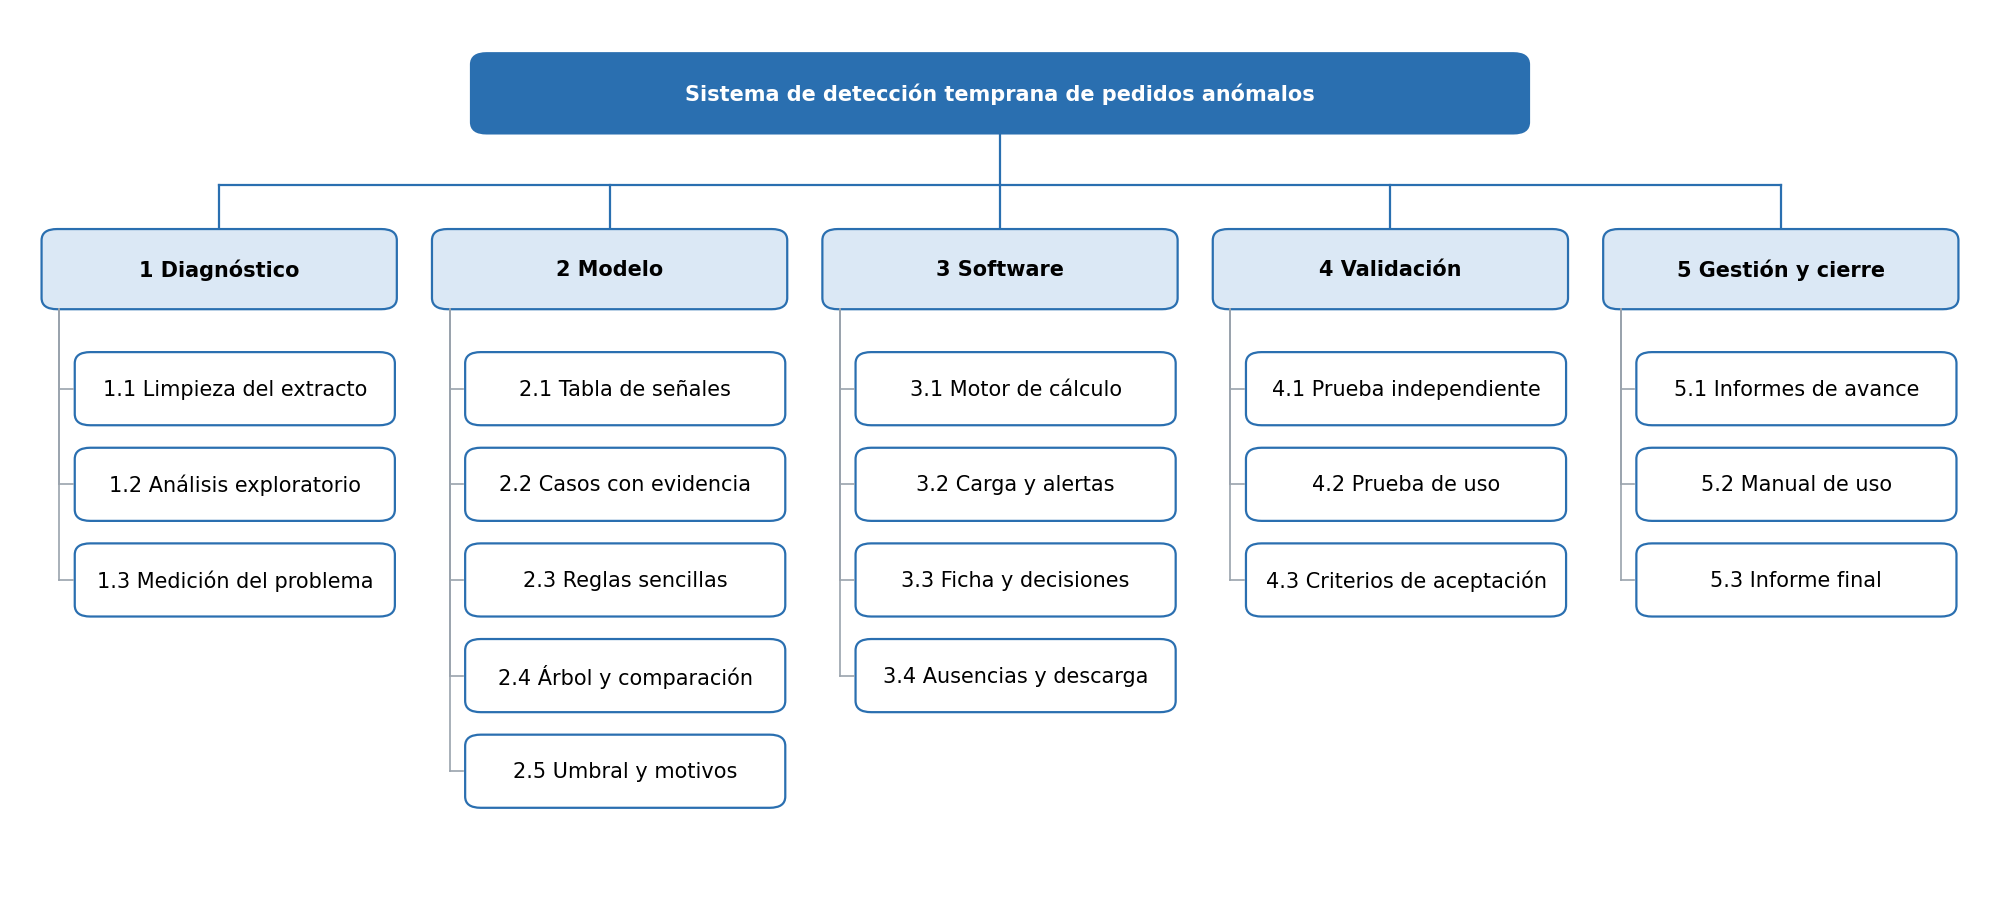
\includegraphics[width=\textwidth]{edt.png}
\caption{Estructura de desglose del trabajo (EDT) del proyecto.}
\label{fig:edt}
\end{figure}

\subsection{Paquetes de trabajo}

\begin{table}[htbp]
\centering
\caption{Paquetes de trabajo, su producto y su esfuerzo estimado. La responsable de todos es la autora del proyecto.}
\label{tab:paquetes}
\small
\begin{tabularx}{\textwidth}{@{}lL{4cm}Ycc@{}}
\toprule
\textbf{Código} & \textbf{Paquete} & \textbf{Producto verificable} & \textbf{Horas} & \textbf{Estado} \\
\midrule
1.1--1.3 & Diagnóstico & Archivo limpio, cifras del problema y programa que las reproduce & 40 & Hecho \\
2.1 & Tabla de señales & Excel con las señales por línea y por semana & 20 & Hecho \\
2.2 & Casos con evidencia & Lista de casos con su etiqueta y la evidencia que la respalda & 24 & En curso \\
2.3 & Reglas sencillas & Métricas por periodo de tres reglas y de la versión por pedido & 16 & Hecho \\
2.4 & Árbol y comparación & Árbol entrenado y comparación con la mejor regla & 20 & Pendiente \\
2.5 & Umbral y motivos & Umbral elegido y frase explicativa por alerta & 12 & Pendiente \\
3.1 & Motor de cálculo & Función que transforma el Excel en la tabla de alertas & 16 & Pendiente \\
3.2--3.4 & Interfaz & Aplicación con carga, alertas, ficha, ausencias y descarga & 40 & Pendiente \\
4.1--4.3 & Validación & Resultados en el periodo independiente y acta de prueba de uso & 24 & Pendiente \\
5.1--5.3 & Gestión y cierre & Informes, manual de uso e informe final & 28 & En curso \\
\midrule
& \textbf{Total} & & \textbf{240} & \\
\bottomrule
\end{tabularx}
\end{table}

\subsection{Entregables y criterios de aceptación}

Cada entregable de primer nivel de la EDT tiene una condición verificable que indica cuándo está terminado y la evidencia que lo demuestra (Tabla~\ref{tab:entregables}). Los criterios detallados del software se encuentran en la Tabla~\ref{tab:aceptacion}.

\begin{table}[htbp]
\centering
\caption{Entregables del proyecto y su criterio de aceptación.}
\label{tab:entregables}
\small
\begin{tabularx}{\textwidth}{@{}L{2.6cm}YL{3.2cm}c@{}}
\toprule
\textbf{Entregable} & \textbf{Se acepta cuando\ldots} & \textbf{Evidencia} & \textbf{Semana} \\
\midrule
1 Diagnóstico & El programa reproduce desde el archivo original las cifras del problema & Salidas \texttt{01\_limpio.xlsx} y Sección~\ref{sec:datos} & 2 \\
2 Modelo & Existe una decisión documentada entre árbol y regla, tomada con el periodo de validación y con al menos 20 errores confirmados & Registro de casos con evidencia y comparación por periodo & 8 \\
3 Software & Cumple los 9 criterios de aceptación de la Tabla~\ref{tab:aceptacion} & Archivo de salida y acta de prueba & 11 \\
4 Validación & Las métricas se calcularon una sola vez sobre el periodo independiente y se reportan frente a sus metas & Informe de resultados & 12 \\
5 Gestión y cierre & El asesor aprueba el informe final y la jefatura recibe el manual de uso & Acta de entrega & 12 \\
\bottomrule
\end{tabularx}
\end{table}

\subsection{Resultados esperados}

Al cierre de la semana 12 se espera contar con tres resultados. El primero es un \textbf{software} que, a partir del archivo exportado y en menos de un minuto, entregue las líneas a revisar con su motivo y con varios días de anticipación respecto de la entrega. El segundo es una \textbf{evaluación} del método sobre un periodo que no se usó para construirlo, expresada en la proporción de alertas que resultaron ser errores confirmados y en la proporción de errores que el método detectó. El tercero es un \textbf{registro de casos} revisados con evidencia, que permita seguir mejorando el método con el uso. Si la evaluación muestra que el árbol de decisión no supera a la mejor regla sencilla, el software se entregará igualmente sobre esa regla, y ese hallazgo se reportará como resultado.

\section{Cronograma}
\label{sec:cronograma}

\subsection{Diagrama de Gantt preliminar}

El proyecto se organiza en doce semanas. La Figura~\ref{fig:gantt} muestra las tareas, su duración y su estado al cierre de la semana 6. El detalle de cada paso se encuentra en la Tabla~\ref{tab:pasos}.

\begin{figure}[htbp]
\centering
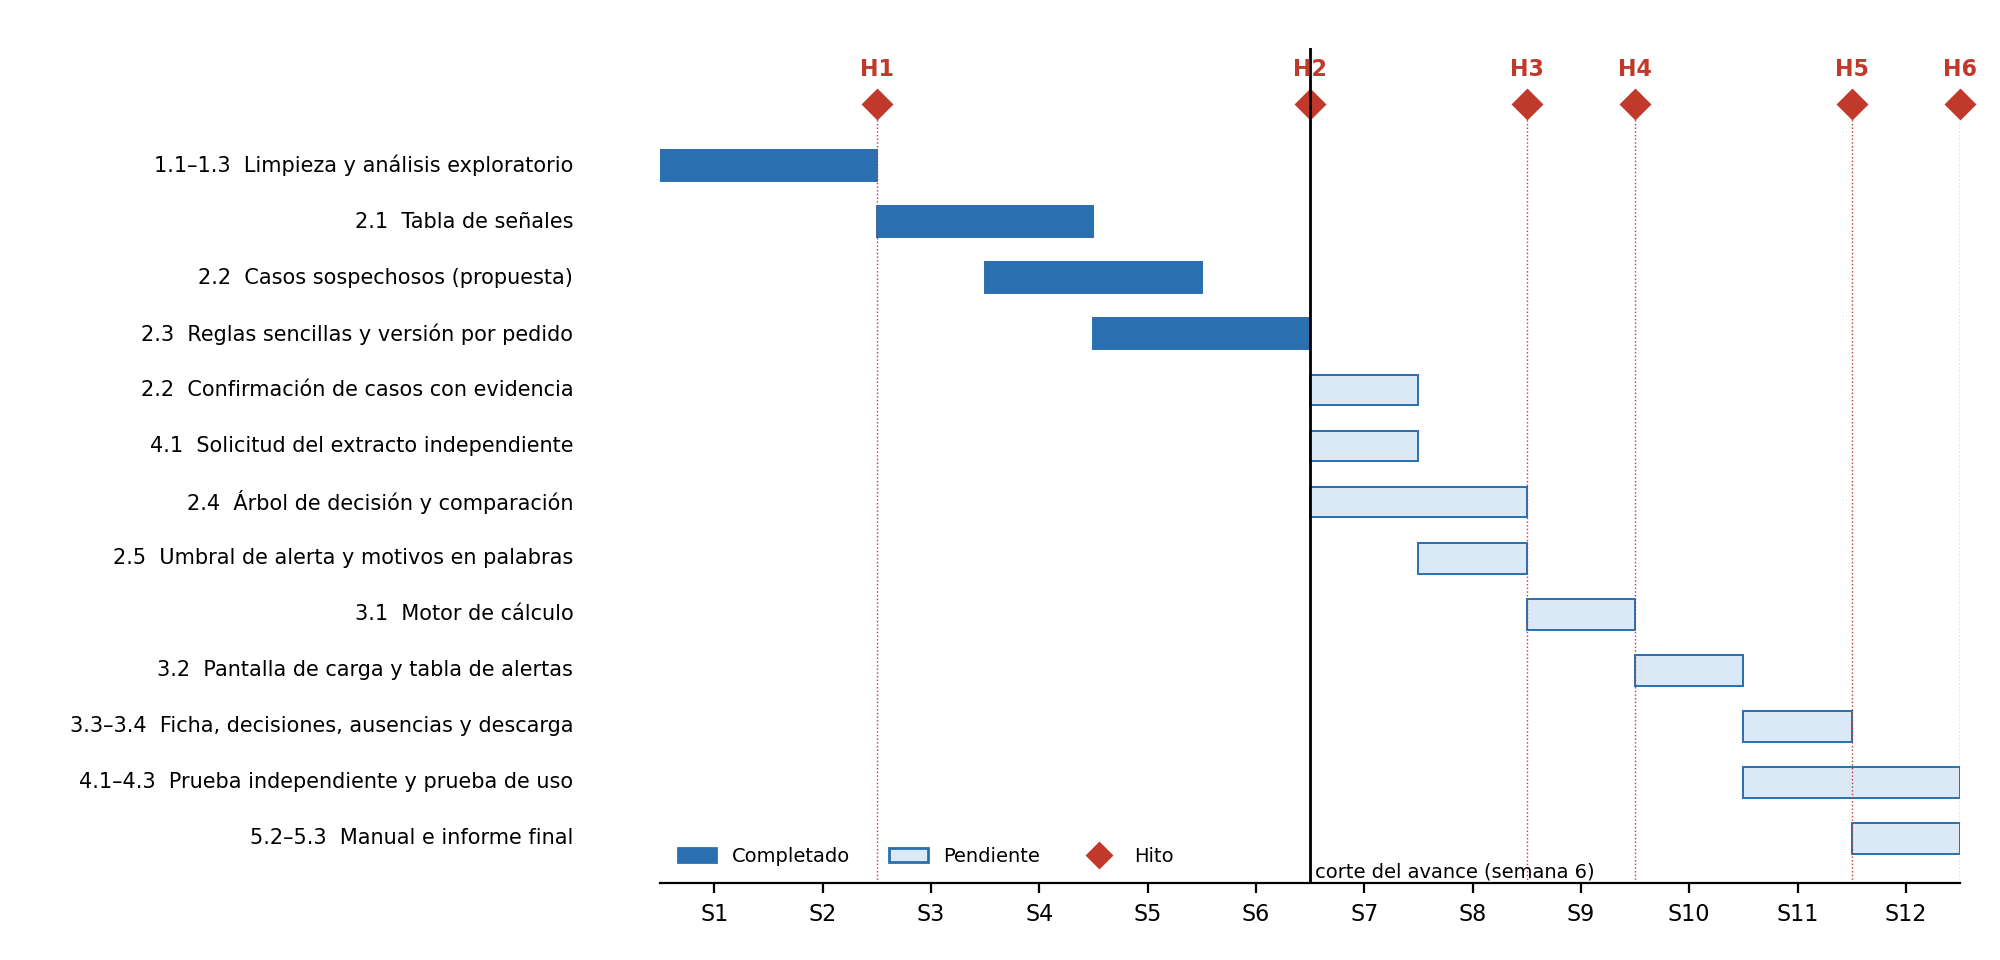
\includegraphics[width=\textwidth]{gantt.png}
\caption{Diagrama de Gantt preliminar. Las barras oscuras están completadas; la línea vertical marca el corte de este avance.}
\label{fig:gantt}
\end{figure}

El cronograma incorpora un ajuste respecto del plan original: la decisión sobre el árbol de decisión se traslada de la semana 7 a la 8, porque antes es necesario confirmar los casos con evidencia y recalcular las señales con la información disponible en cada momento. El desplazamiento se absorbe dentro de la semana 8 y no modifica la fecha de entrega. La secuencia que determina esa fecha es la confirmación de casos, el entrenamiento del árbol, la elección del umbral y la construcción del motor de cálculo; su eslabón más frágil es la confirmación de casos, porque depende de los correos que conserva el área de planeamiento.

\subsection{Identificación de hitos}

La Tabla~\ref{tab:hitos} indica, para cada hito, la decisión que se toma y quién la toma.

\begin{table}[htbp]
\centering
\caption{Hitos del proyecto.}
\label{tab:hitos}
\small
\begin{tabularx}{\textwidth}{@{}lcYL{2.6cm}l@{}}
\toprule
\textbf{Hito} & \textbf{Semana} & \textbf{Decisión que se toma} & \textbf{Quién decide} & \textbf{Estado} \\
\midrule
H1 Diagnóstico & 2 & El problema está medido y justifica el proyecto & Asesor & Cumplido \\
H2 Línea base fijada & 6 & Se fija la cifra que el modelo debe superar & Autora & Cumplido \\
H3 ¿Árbol o regla? & 8 & Se decide si el árbol aporta frente a la mejor regla & Autora, con visto bueno del asesor & Pendiente \\
H4 Motor operativo & 9 & El cálculo funciona de punta a punta sin pantallas & Autora & Pendiente \\
H5 Aplicación completa & 11 & La herramienta está lista para la prueba de uso & Autora & Pendiente \\
H6 Entrega final & 12 & Se acepta el prototipo según los criterios de la Tabla~\ref{tab:aceptacion} & Asesor y jefatura & Pendiente \\
\bottomrule
\end{tabularx}
\end{table}

\section{Presupuesto}
\label{sec:presupuesto}

\subsection{Estimación preliminar de costos}

El proyecto no requiere compras de equipos ni licencias: todas las herramientas son de uso libre y el volumen de datos se procesa en una computadora personal. Su costo es, principalmente, el tiempo de las personas que participan. La Tabla~\ref{tab:presupuesto} lo valoriza para dar una idea del esfuerzo que representa. Ninguna partida implica un desembolso adicional para la empresa, salvo las horas que destinen la analista y la jefatura.

\begin{table}[htbp]
\centering
\caption{Estimación preliminar de costos del proyecto (12 semanas).}
\label{tab:presupuesto}
\small
\begin{tabularx}{\textwidth}{@{}YL{2.8cm}rr@{}}
\toprule
\textbf{Partida} & \textbf{Cantidad} & \textbf{Costo unitario (S/)} & \textbf{Total (S/)} \\
\midrule
\multicolumn{4}{@{}l}{\textit{Personas}} \\
Practicante (autora) & 240 h & 12 & 2\,880 \\
Asesor académico & 12 h & 80 & 960 \\
Analista de planeamiento (revisión de casos y prueba de uso) & 8 h & 25 & 200 \\
Jefatura de planeamiento (hitos y cierre) & 2 h & 50 & 100 \\
\midrule
\multicolumn{4}{@{}l}{\textit{Equipos y servicios}} \\
Computadora personal (uso prorrateado de 3 meses) & 3 meses & 83 & 250 \\
Internet y energía & 3 meses & 60 & 180 \\
Software (Python, \texttt{pandas}, \texttt{scikit-learn}, Streamlit, \LaTeX) & -- & 0 & 0 \\
\midrule
\textbf{Línea base de costos} & & & \textbf{4\,570} \\
Reserva de contingencia (10\,\%) & & & 457 \\
\midrule
\textbf{Presupuesto del proyecto} & & & \textbf{5\,027} \\
Reserva de gestión (5\,\%, fuera de la línea base) & & & 229 \\
\midrule
\textbf{Total con reservas} & & & \textbf{5\,256} \\
\bottomrule
\end{tabularx}
\end{table}

La \textbf{reserva de contingencia} cubre riesgos ya identificados en la Sección~\ref{sec:riesgos-final}, en particular que la confirmación de casos o la obtención del extracto independiente tomen más horas de las previstas; su uso lo autoriza la autora y se registra con su motivo. La \textbf{reserva de gestión} cubre imprevistos que no figuran en el registro de riesgos, como un cambio de alcance solicitado por la empresa; su uso requiere la aprobación del asesor.

Como referencia, el valor potencial en riesgo estimado en la Sección~\ref{sec:datos} es de alrededor de S/~3\,200 al mes. Esta cifra no es una pérdida comprobada (Sección~\ref{sec:av-terminos}), por lo que no se usa para calcular un retorno de la inversión; solo indica que el orden de magnitud del problema es comparable al costo total del proyecto.

\subsection{Supuestos utilizados}

\begin{itemize}
\item El esfuerzo de la practicante es de 20 horas por semana durante 12 semanas, valorizado en S/~12 por hora, una cifra cercana a la subvención mensual de prácticas.
\item El asesor dedica una hora por semana, valorizada a una tarifa referencial de docencia de S/~80 por hora.
\item La analista dedica 6 horas a confirmar casos y 2 a la prueba de uso; la jefatura, 2 horas a hitos y cierre. Ambas se valorizan con tarifas horarias referenciales, no con salarios reales.
\item La computadora es propia, con un valor de S/~3\,000 y una vida útil de 36 meses; se imputa el uso de 3 meses.
\item No se contratan servicios en la nube ni licencias: el software corre en el equipo del usuario.
\item Las tarifas son supuestos de orden de magnitud y deberán validarse con el área si el presupuesto se usa para decidir.
\end{itemize}

\section{Riesgos}
\label{sec:riesgos-final}

\subsection{Lista preliminar de riesgos}

La Tabla~\ref{tab:riesgos} actualiza la matriz del primer entregable con lo observado en la ejecución y con la retroalimentación del asesor. Cada riesgo se describe como una condición y su consecuencia, con la señal que permite anticiparlo.

\begin{table}[htbp]
\centering
\caption{Lista de riesgos con probabilidad (P) e impacto (I) de 1 a 5, y estrategia de respuesta.}
\label{tab:riesgos}
\footnotesize
\begin{tabularx}{\textwidth}{@{}lL{4.2cm}ccL{2.1cm}Y@{}}
\toprule
\textbf{ID} & \textbf{Si\ldots{} entonces\ldots} & \textbf{P} & \textbf{I} & \textbf{Estrategia} & \textbf{Respuesta y señal temprana} \\
\midrule
R1 & Si no se reúnen 20 errores confirmados, el modelo no tendrá de qué aprender & 5 & 4 & Mitigar & Confirmar los 78 casos con correos en la semana 7. Señal: hoy hay un solo error confirmado \\
R2 & Si el modelo usa información que no existe al alertar, su desempeño real será menor & 4 & 4 & Evitar & Calcular todas las señales con lo registrado hasta cada momento. Señal: la versión por pedido ya rinde menos que la semanal \\
R3 & Si no se obtiene un extracto posterior, no habrá evaluación independiente & 3 & 5 & Mitigar & Solicitarlo en la semana 7; si no llega, reservar las dos últimas semanas del extracto actual sin usarlas \\
R4 & Si el árbol se ajusta demasiado a pocas semanas, fallará con datos nuevos & 3 & 4 & Mitigar & Limitar su profundidad y compararlo solo en validación. Señal: gran diferencia entre ajuste y validación \\
R5 & Si las campañas generan alertas correctas pero inútiles, el analista dejará de mirarlas & 3 & 4 & Mitigar & Usar el movimiento común de la cadena. Señal: más de 10\,\% de series en alza la misma semana \\
R6 & Si el historial contiene errores, la referencia quedará inflada & 3 & 3 & Mitigar & Usar medianas y recalcular sin los casos confirmados \\
R7 & Si el software no se adopta, se volverá a la revisión manual & 2 & 4 & Mitigar & Interfaz de un solo paso y criterio de aceptación 9 \\
R8 & Si cambia el formato del archivo exportado, el programa fallará & 2 & 3 & Aceptar & Verificar columnas al inicio con un mensaje explícito \\
\bottomrule
\end{tabularx}
\end{table}

\subsection{Matriz de probabilidad e impacto}

\begin{figure}[htbp]
\centering
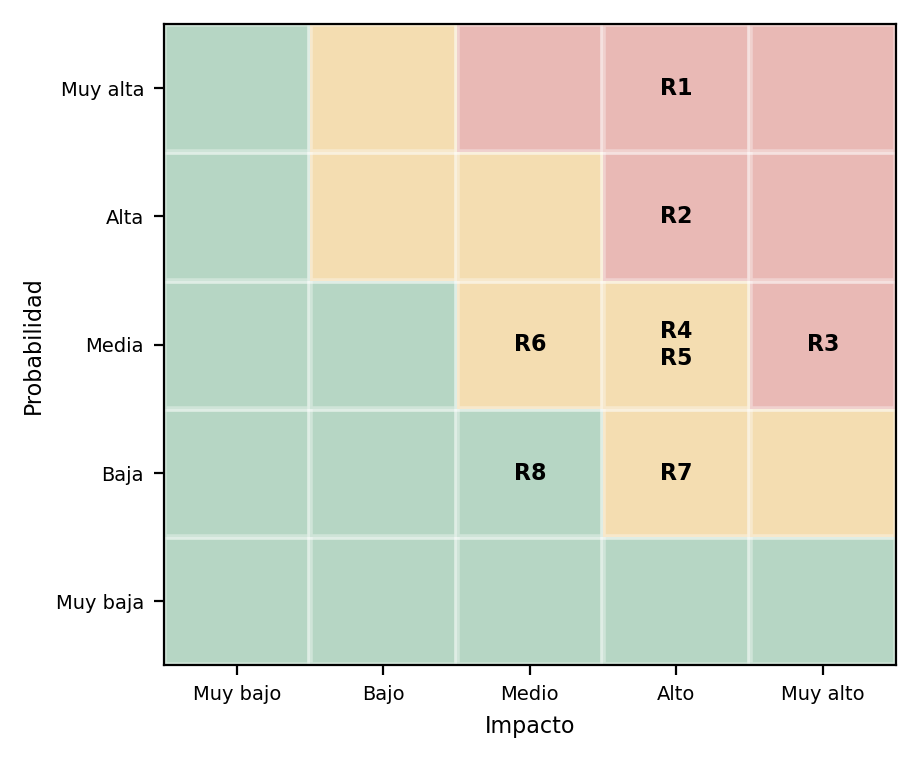
\includegraphics[width=0.55\textwidth]{matriz_riesgos.png}
\caption{Matriz de probabilidad e impacto. Los riesgos en rojo requieren respuesta inmediata; los ámbar, seguimiento semanal.}
\label{fig:matriz}
\end{figure}

\subsection{Estrategias de respuesta}

Los riesgos R1, R2 y R3 son los que más pueden afectar el resultado del proyecto, ya que tienen que ver con cuántos errores se confirman, qué información se usa para alertar y en qué periodo se mide el desempeño. Por eso se atienden en la semana 7, antes de entrenar el árbol. Los riesgos R4 a R6 se mitigan con decisiones de diseño ya incorporadas al método. El R7 se gestiona con la prueba de uso de la semana 12 y el R8 se acepta, porque su impacto es acotado y su detección inmediata.

\section{Indicadores}
\label{sec:kpis}

La Tabla~\ref{tab:alineacion} muestra cómo cada elemento del plan responde al anterior: el problema da lugar a la causa raíz, esta al objetivo, el objetivo a un entregable y el entregable a un indicador que permite verificarlo.

\begin{table}[htbp]
\centering
\caption{Alineación entre problema, objetivos, entregables e indicadores.}
\label{tab:alineacion}
\footnotesize
\begin{tabularx}{\textwidth}{@{}YYL{2.4cm}L{2.6cm}@{}}
\toprule
\textbf{Causa que se ataca} & \textbf{Objetivo específico} & \textbf{Entregable} & \textbf{Indicador} \\
\midrule
No hay un valor de referencia por tienda & 2. Valor esperado con información disponible & 2 Modelo & Error de la referencia \\
La revisión es visual y no prioriza & 4. Elegir el método que alerta mejor & 2 Modelo & Precisión y exhaustividad \\
Las alertas llegan tarde o no se revisan & 5. Software con motivo y anticipación & 3 Software & Carga de alertas y anticipación \\
No se sabe si el control funciona & 3 y 6. Casos confirmados y evaluación independiente & 4 Validación & Errores confirmados \\
\bottomrule
\end{tabularx}
\end{table}


La Tabla~\ref{tab:indicadores} define los indicadores con que se medirá el proyecto. Se distinguen los indicadores de \emph{resultado}, que dicen si el problema se está resolviendo, de los indicadores \emph{líderes}, que avisan con anticipación si el resultado está en riesgo.

\begin{table}[htbp]
\centering
\caption{Indicadores clave del proyecto.}
\label{tab:indicadores}
\footnotesize
\begin{tabularx}{\textwidth}{@{}L{2.6cm}YL{1.6cm}L{1.5cm}L{1.6cm}@{}}
\toprule
\textbf{Indicador} & \textbf{Cómo se calcula} & \textbf{Meta} & \textbf{Tipo} & \textbf{Hoy} \\
\midrule
Precisión de las alertas & Alertas que resultan ser errores confirmados / alertas emitidas & $\geq 70$\,\% & Resultado & Por medir \\
Exhaustividad & Errores confirmados detectados / errores confirmados & $\geq 80$\,\% & Resultado & 1 de 1 \\
Carga de alertas & Alertas emitidas por semana & 2 a 5 & Resultado & 2 a 6 \\
Anticipación & Días entre la alerta y la fecha de entrega (mediana) & $\geq 3$ días & Resultado & 3 a 5 \\
Tiempo de proceso & Segundos entre la carga del archivo y el resultado & $< 60$ s & Resultado & 17 s (prototipo) \\
Errores confirmados & Casos con evidencia operativa acumulados & $\geq 20$ & Líder & 1 \\
\bottomrule
\end{tabularx}
\end{table}

\section{Retroalimentación incorporada}\label{sec:retro}

El asesor planteó delimitar mejor el problema: que el pedido no lo envíe el usuario de tienda sino directamente un software. La idea ataca el error en su origen, porque si nadie digita no hay nada que digitar mal. Se evaluó y se optó por otra delimitación, porque las dos propuestas automatizan cosas de naturaleza distinta \segun{y solo una conviene automatizar:}{y solo una corresponde al proveedor:} el envío del pedido es un proceso de cara al cliente, la detección de errores es un control interno del proveedor.

\begin{table}[htbp]
\centering
\caption{Automatizar el pedido frente a automatizar la detección.}
\label{tab:retro}
\small
\begin{tabularx}{\textwidth}{@{}L{3cm}YY@{}}
\toprule
 & \textbf{Automatizar el pedido} & \textbf{Automatizar la detección} \\
\midrule
Dónde corre & En el proceso de compras del cliente & En el proveedor, sobre su propio archivo \\
Permisos & Compras y TI del cliente & Ninguno \\
Al replicarlo con otro cliente & Hay que rehacerlo: otro ERP, otro formato, otro calendario & Funciona igual: el dato de entrada es del proveedor \\
Si se equivoca & El pedido errado lo emitió el proveedor & Se pierde una alerta; el pedido sigue siendo del cliente \\
Sobre la relación & Elimina el contacto semanal & Le da contenido \\
\bottomrule
\end{tabularx}
\end{table}

Automatizar el flujo con el cliente tiene tres costos. El primero es que el esfuerzo no se acumula: el pedido cambia de cliente a cliente y con la temporada, de modo que habría que construir y mantener una integración por cada cadena, sin reutilizar nada con la siguiente. El segundo es que ese pedido semanal es la línea directa con el cliente, el momento en que el proveedor se entera de lo que la tienda cree que va a necesitar; ahí aparecen las señales de que algo cambió, desde una caída sostenida hasta el reparto del volumen con otro proveedor. Un sistema que genera los pedidos por su cuenta deja de recibir esa señal y se enteraría tarde, cuando el volumen ya bajó. El tercero es un traslado de responsabilidad: hoy, si la cantidad está mal, el error es del cliente y el proveedor tiene con qué sustentarlo; si el proveedor emitiera los pedidos, cualquier sobre-despacho pasaría a ser error propio, con la discusión comercial y la devolución a cuenta suya.

El control interno no tiene ninguno de esos costos. Corre sobre datos que el proveedor ya tiene, sirve igual para cualquier cliente que emita pedidos, y no sustituye la conversación sino que le da contenido: en lugar de un correo que dice «su pedido parece alto», el área envía la cantidad solicitada, la esperada según el historial de esa tienda y el motivo. \segun{Eso fideliza más que hacerle el pedido, porque demuestra que alguien está mirando sus números. La regla que ordena la decisión es automatizar donde el proceso es estable y propio, y dejarlo fuera donde es variable y compartido.}{Esto aporta más a la relación con el cliente que emitir el pedido por él. En resumen, se automatiza el proceso que pertenece al proveedor y es estable, y se deja fuera el que es compartido con el cliente y cambia con cada cadena.}

La observación sí amplió el alcance en un punto. Si el software estima la demanda esperada de cada tienda, también puede detectar la ausencia de pedido: una tienda que debía pedir y no pidió. Ese caso no estaba contemplado y se incorporó según la Sección~\ref{sec:ausencias}.

\iffinal
\subsection{Segunda revisión del asesor}

La revisión del avance planteó seis observaciones. La Tabla~\ref{tab:av-retro} resume cómo se incorporó cada una y en qué sección se desarrolla. Estas observaciones modificaron tres aspectos del proyecto: qué información puede usar el método, qué se considera un error y sobre qué periodo se mide el desempeño.

\begin{table}[htbp]
\centering
\caption{Observaciones de la segunda revisión y su incorporación.}
\label{tab:av-retro}
\small
\begin{tabularx}{\textwidth}{@{}L{4.8cm}YL{1.6cm}@{}}
\toprule
\textbf{Observación} & \textbf{Cambio realizado} & \textbf{Sección} \\
\midrule
Cada variable debe conocerse al emitir la alerta & Se clasificaron las variables por disponibilidad y se construyó una versión que evalúa cada línea con lo sabido ese día & \ref{sec:av-tiempo}, \ref{sec:av-por-pedido} \\
Distinguir desviación de error confirmado & Terminología de tres niveles: desviación, caso sospechoso y error confirmado & \ref{sec:av-terminos} \\
Distinguir valor en riesgo de pérdida ocurrida & Los S/~3\,200 mensuales se presentan como valor potencial en riesgo & \ref{sec:av-terminos}, \ref{sec:datos} \\
Validar etiquetas con evidencia operativa & Cada error exige una fuente documentada; las modificaciones de cantidad dejan de contarse como errores & \ref{sec:av-marcado} \\
Pasar del análisis semanal a alertas por pedido & Procedimiento en tres etapas, ya implementado en el prototipo & \ref{sec:av-pedido} \\
Reservar un periodo independiente y moderar conclusiones & Periodos de ajuste, validación y prueba; las cifras se reportan como preliminares & \ref{sec:av-periodos} \\
\bottomrule
\end{tabularx}
\end{table}
\else
\section{Estado actual del proyecto}
\label{sec:estado-e1}

El proyecto se encuentra en la \textbf{etapa de análisis}. Lo que este entregable presenta es el problema delimitado, medido y con un método de detección probado sobre los datos históricos. La construcción del software todavía no ha empezado: corresponde a los pasos 8 a 12 del plan de trabajo.

Lo que ya está resuelto es lo siguiente. El problema dejó de ser una queja y pasó a tener cifras: 54 casos de cantidad repetida, 17 desviaciones relevantes en nueve semanas y alrededor de S/~3\,200 mensuales en producto despachado por encima de lo esperado. El criterio de detección se probó contra un caso que la operación ya había identificado por su cuenta, el de la tienda de ATE, y lo reencontró sin ayuda. Y el principal riesgo del método, confundir un feriado con un error, quedó resuelto dentro del propio cálculo mediante la separación entre el movimiento común de la cadena y el de cada tienda, sin depender de que alguien recuerde qué pasó una semana determinada.

Lo que falta es lo que va de la semana 3 en adelante. El árbol de decisión aún no está entrenado, los cinco parámetros de la Tabla~\ref{tab:hiper} tienen valores iniciales pero no ajustados con validación temporal, y el software existe como especificación y no como programa. Las métricas comprometidas en la Tabla~\ref{tab:indicadores} son metas y todavía no resultados.
\fi

% ============================================================
%  Sección 6 — Avance del proyecto, semanas 3 a 6
%  Redacción académica en lenguaje accesible.
%  Incorpora la retroalimentación del asesor sobre el Entregable 1.
% ============================================================

\section{Avance del proyecto}
\label{sec:avance}

Entre la tercera y la sexta semana se completaron los pasos 2, 3 y 4 del plan de trabajo (Tabla~\ref{tab:pasos}) y se revisaron las cifras del paso 1. El avance ya incorpora las observaciones del asesor resumidas en la Sección~\ref{sec:retro}, y los primeros apartados explican cómo se aplicó cada una.

Los resultados se obtuvieron con un programa en Python que lee el archivo exportado del sistema de compras sin modificarlo, por lo que pueden repetirse con cualquier exportación del mismo formato. Las capturas de los archivos de salida y del código están en el Anexo~\ref{sec:anexo}. Como se trabajó con pocas semanas y con etiquetas aún no confirmadas, los resultados son preliminares.

\subsection{Retroalimentación del asesor y cómo se incorpora}
\label{sec:av-retro}

El asesor señaló seis aspectos, resumidos en la Tabla~\ref{tab:av-retro}; los apartados siguientes los desarrollan.

\iffinal\else
\begin{table}[htbp]
\centering
\caption{Observaciones del asesor y su incorporación.}
\label{tab:av-retro}
\small
\begin{tabularx}{\textwidth}{@{}L{5.2cm}Y@{}}
\toprule
\textbf{Observación} & \textbf{Cómo se incorpora} \\
\midrule
Cada variable debe conocerse en el momento de emitir la alerta, antes del despacho & Se clasifican las variables según cuándo están disponibles y se excluyen del modelo las que usan información posterior (Sección~\ref{sec:av-tiempo}) \\
Distinguir una desviación respecto del historial de un error confirmado & Se adopta una terminología de tres niveles, que son desviación, caso sospechoso y error confirmado (Sección~\ref{sec:av-terminos}) \\
Distinguir el valor potencial en riesgo de una pérdida efectivamente ocurrida & La cifra de S/~3\,200 mensuales se presenta como valor potencial en riesgo, no como pérdida (Sección~\ref{sec:av-terminos}) \\
Validar las etiquetas con evidencia operativa, pues una modificación puede ser legítima & Las líneas rectificadas dejan de considerarse errores automáticamente y cada etiqueta exige una fuente documentada (Sección~\ref{sec:av-marcado}) \\
Explicar el paso del análisis semanal a alertas por pedido & Se describe el procedimiento para evaluar cada línea en el momento en que se registra (Sección~\ref{sec:av-pedido}) \\
Reservar un periodo independiente de evaluación y moderar las conclusiones & Se separan tres periodos y se reserva un extracto nuevo que no se usará hasta la evaluación final (Sección~\ref{sec:av-periodos}) \\
\bottomrule
\end{tabularx}
\end{table}
\fi

\subsubsection{Qué información existe en el momento de alertar}
\label{sec:av-tiempo}

En el archivo, cada línea se registra en promedio cinco días antes de su fecha de entrega, y el 80\,\% se registra con menos de una semana de anticipación. Esto significa que, cuando se registra una línea, todavía no se conocen las demás líneas que la misma tienda cargará esa semana, ni lo que pedirá la semana siguiente. La Tabla~\ref{tab:av-disponibilidad} explica qué significa cada variable y si está disponible en ese momento.

\begin{table}[htbp]
\centering
\caption{Variables del método, su significado y su disponibilidad al emitir la alerta.}
\label{tab:av-disponibilidad}
\footnotesize
\begin{tabularx}{\textwidth}{@{}L{2.7cm}YL{1.6cm}L{3.1cm}@{}}
\toprule
\textbf{Variable} & \textbf{Qué significa (ejemplo)} & \textbf{¿Disponible al alertar?} & \textbf{Tratamiento} \\
\midrule
Referencia de la tienda & Lo que esa tienda suele pedir de ese producto en una semana, calculado como la mediana de sus últimas cuatro semanas. \emph{Ej.: en las cuatro semanas previas al 17 de agosto, ATE pidió 216, 126, 108 y 108 panes grandes; su referencia (la mediana) es 117.} & Sí & Se calcula solo con semanas anteriores \\
Variación frente a la semana anterior & Cuánto cambió el pedido respecto de la semana pasada. \emph{Ej.: de 120 a 240 unidades es una variación de +100\,\%.} & Sí & Sin cambios \\
Línea duplicada & Indica si la tienda tiene dos líneas iguales, con el mismo producto, misma fecha de entrega y misma cantidad. Suele ser el mismo pedido cargado dos veces. \emph{Ej.: dos líneas de 180 panes junior para el 05/09.} & Sí, parcialmente & Solo se compara con las líneas ya registradas \\
Peso del producto en el pedido & Qué parte del pedido total de la tienda corresponde a ese producto, comparada con lo usual. \emph{Ej.: el pan grande suele ser el 20\,\% del pedido y esta semana es el 50\,\%.} & Parcialmente & Con lo registrado hasta ese momento \\
Presentaciones que suben juntas & Cuántas de las tres presentaciones (grande, mediano y junior) subieron más de 30\,\% en la misma tienda y semana. Si suben las tres, suele ser demanda real; si sube una sola, es más sospechoso. & Parcialmente & Con lo registrado hasta ese momento \\
Movimiento común de la cadena & Cuánto subieron o bajaron en promedio todas las tiendas esa semana. Permite distinguir un feriado, en que suben todas, de un error, en que sube una sola. \emph{Ej.: en Fiestas Patrias toda la cadena subió alrededor de 11\,\%.} & Parcialmente & Con las tiendas que ya registraron su pedido \\
Lo que la tienda pide la semana siguiente & Si el pedido alto se repite o vuelve a lo normal la semana después. Ayudó en el análisis, pero ese dato todavía no existe cuando hay que alertar. & \textbf{No} & Solo para análisis retrospectivo; fuera del modelo \\
\bottomrule
\end{tabularx}
\end{table}

Esto afecta a dos elementos del primer entregable. La última fila de la Tabla~\ref{tab:firma} usa el comportamiento de la semana siguiente; sirvió para diferenciar una campaña de un error, pero no puede usarse para alertar. Lo mismo ocurre con el parámetro de reversión de la Tabla~\ref{tab:hiper}, que queda solo para revisar casos pasados. Además, las reglas semanales de esta sección usan semanas completas, por lo que en operación se reemplazan por la versión por pedido.

\subsubsection{Desviación, caso sospechoso y error confirmado}
\label{sec:av-terminos}

En el primer entregable se usaron como sinónimos «desviación», «anomalía» y «error». A partir de este avance se usan tres términos distintos.

\begin{itemize}
\item \emph{Desviación}. Es un pedido que se aleja del patrón histórico de la tienda. No implica que esté mal; puede deberse a una promoción, a un evento local o a un cambio de necesidad.
\item \emph{Caso sospechoso}. Es una desviación que se debe revisar porque presenta al menos una de las siguientes características.
\begin{itemize}
\item la tienda subió más de 80\,\% sobre su referencia mientras el resto de la cadena no subió (no es feriado ni campaña);
\item subió una o dos presentaciones, pero no las tres a la vez, lo que no se parece a un aumento real de demanda;
\item tiene una línea duplicada, con el mismo producto, fecha de entrega y cantidad;
\item una línea es varias veces más grande que las líneas habituales de esa tienda y producto;
\item el pedido cayó más de 60\,\% respecto de su referencia, lo que puede indicar un pedido incompleto.
\end{itemize}
\item \emph{Error confirmado}. Es un caso sospechoso respaldado por evidencia operativa, por ejemplo un correo en que el área o la tienda reconoce el error.
\end{itemize}

Con esta distinción, los 17 casos y los S/~3\,200 mensuales de la Tabla~\ref{tab:exceso} corresponden a desviaciones. Esa cifra es un valor potencial en riesgo, es decir, el valor del producto despachado por encima de lo esperado si todas las desviaciones fueran errores. La pérdida real será menor y se podrá estimar cuando se sepa cuántas desviaciones se confirman y qué parte del exceso no se recuperó por otra vía.

\subsubsection{Del análisis semanal a la alerta por pedido}
\label{sec:av-pedido}

El análisis exploratorio agrupó los pedidos por tienda, producto y semana, pero la herramienta final debe evaluar cada línea cuando se registra. Para ello se combinan tres comparaciones.

\begin{enumerate}
\item La referencia de la tienda sigue siendo semanal y se calcula con las semanas anteriores, que ya se conocen.
\item Al registrarse una línea, se suma con las líneas de la misma tienda y producto ya cargadas para esa semana, y el acumulado se compara con lo que la tienda suele llevar pedido hasta ese día.
\item La línea se compara también con el tamaño habitual de las líneas de esa tienda y producto, para detectar errores que en el total semanal no se notan (Sección~\ref{sec:av-marcado}).
\end{enumerate}

Así, la alerta corresponde a una línea concreta y puede emitirse el mismo día del registro, varios días antes de la entrega.

\subsubsection{Periodos de ajuste, validación y prueba}
\label{sec:av-periodos}

Hasta ahora el extracto se dividía en dos partes, hasta el 10 de agosto para ajustar y las tres semanas siguientes para evaluar. Sin embargo, esas semanas también se revisaron al definir los casos sospechosos, así que no eran del todo independientes. Se adopta entonces una división en tres periodos, que deja las dos últimas semanas completas sin usar hasta el final.

\begin{itemize}
\item Ajuste (13 de julio al 3 de agosto), para construir el método y fijar sus umbrales.
\item Validación (10 y 17 de agosto), para comparar alternativas y elegir parámetros.
\item Prueba (24 y 31 de agosto), que se mide una sola vez, con el método ya definido.
\end{itemize}

La semana del 7 de septiembre está incompleta y no se usa. Además, se pedirá al área de planeamiento un extracto posterior al 11 de septiembre para confirmar los resultados con pedidos nuevos. La precisión y la exhaustividad se medirán en el periodo de prueba cuando haya etiquetas confirmadas.

\subsection{Resumen del estado del proyecto}
\label{sec:av-resumen}

El proyecto se encuentra en la semana 6 de 12, y los productos comprometidos hasta esta semana están terminados. Lo que todavía no se puede afirmar es si las alertas alcanzarán la precisión buscada, porque falta confirmar los casos de error. La Tabla~\ref{tab:av-estado} resume la situación.

\begin{table}[htbp]
\centering
\caption{Estado del proyecto al cierre de la semana 6 de 12. La columna «Semana» indica cuándo debe cumplirse cada meta. La precisión y la exhaustividad se medirán en el periodo de prueba cuando haya etiquetas confirmadas.}
\label{tab:av-estado}
\small
\begin{tabularx}{\textwidth}{@{}YL{1.9cm}cL{2.3cm}L{2.2cm}@{}}
\toprule
\textbf{Aspecto evaluado} & \textbf{Meta} & \textbf{Semana} & \textbf{Situación en la semana 6} & \textbf{Estado} \\
\midrule
Productos de los pasos 1 a 4 & 4 de 4 & 6 & 4 de 4 & \textcolor{green!50!black}{\textbf{Cumplido}} \\
Errores confirmados con evidencia operativa & 20 o más & 7 & 1 (caso ATE) & \textcolor{orange!85!black}{\textbf{En camino}} \\
Alertas por semana (acumulado de la semana) & Entre 2 y 5 & 8 & 4,0 & \textcolor{green!50!black}{\textbf{En rango}} \\
Alertas que coinciden con un caso sospechoso & 70\,\% o más & 12 & Por medir & \textcolor{orange!85!black}{\textbf{Pendiente}} \\
Casos sospechosos que el método detecta & 80\,\% o más & 12 & Por medir & \textcolor{orange!85!black}{\textbf{Pendiente}} \\
\bottomrule
\end{tabularx}
\end{table}

Por ahora solo hay un error confirmado por escrito (ATE); los demás son casos sospechosos. Por eso, en esta etapa los métodos se prueban con casos conocidos (Sección~\ref{sec:av-casos}) y la medición de precisión y exhaustividad queda para cuando haya más errores confirmados.

\subsection{Revisión de la limpieza de datos}
\label{sec:av-limpieza}

El programa de limpieza reprodujo casi todas las cifras de la Sección~\ref{sec:anuladas}, entre ellas 10\,374 líneas vigentes, 385 anuladas con reemplazo y 119 líneas duplicadas. Cambiaron dos valores.

Las líneas anuladas que se reemplazaron por otra cantidad pasan de 27 a 23. Cuando una tienda tiene varias líneas del mismo producto el mismo día, no es evidente cuál reemplazó a cuál; el programa toma la primera según el número de orden y posición.

Las observaciones evaluables bajan de 1\,554 a 1\,371 porque se excluyó la última semana. El archivo termina un viernes y esa semana no tiene los pedidos del sábado, por lo que aparentaba una caída general.

\subsection{Paso 2: la tabla de señales}
\label{sec:av-senales}

Para cada tienda, producto y semana se calcularon las ocho señales de la Tabla~\ref{tab:variables}. Estas indican cuánto se aleja el pedido de lo que la tienda suele pedir, cuánto cambió frente a la semana anterior, si hay una línea repetida, si subieron las tres presentaciones y si toda la cadena se movió en la misma dirección. Esta versión usa semanas completas; la versión por pedido se describe en la Sección~\ref{sec:av-por-pedido}.

\begin{figure}[htbp]
\centering
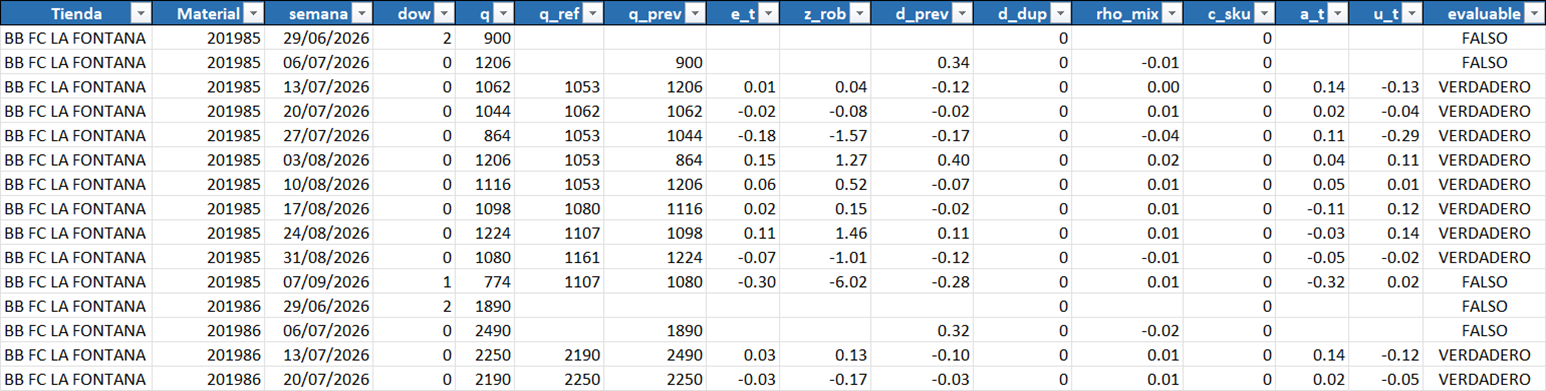
\includegraphics[width=\textwidth]{xl_02_senales.png}
\caption{Captura de \texttt{salidas/02\_senales.xlsx} abierto en Excel, con una fila por tienda, producto y semana con sus señales. El procedimiento que la genera está en el Algoritmo~\ref{alg:senales}.}
\label{fig:av-cap-senales}
\end{figure}

La tabla tiene 1\,371 filas evaluables. La semana del 27 de julio vuelve a mostrar un alza de toda la cadena, que coincide con Fiestas Patrias. La semana del 13 de julio muestra el mismo comportamiento sin un motivo conocido, y se consultará al área de planeamiento. El pedido de ATE del 17 de agosto vuelve a aparecer marcado.

\subsection{Paso 3: casos sospechosos y su validación}
\label{sec:av-marcado}

El archivo no indica qué pedidos estuvieron mal, así que la lista de errores se construye en dos pasos. Primero, el programa selecciona pedidos sospechosos y propone una etiqueta. Después, cada propuesta se confirma o descarta con evidencia operativa.

Se seleccionaron 78 pedidos por tres motivos, que son un alza solo en esa tienda, una línea duplicada o una caída brusca. Se propone como posible error cuando la tienda subió sola, sin que subieran las demás tiendas ni sus otras presentaciones, o cuando hay una línea duplicada con un alza importante (Tabla~\ref{tab:av-candidatos}).

\begin{table}[htbp]
\centering
\caption{Pedidos sospechosos según el motivo y la etiqueta propuesta.}
\label{tab:av-candidatos}
\small
\begin{tabular}{@{}lrr@{}}
\toprule
\textbf{Motivo} & \textbf{Posible error} & \textbf{Probablemente normal} \\
\midrule
Alza que solo afectó a la tienda & 8 & 8 \\
Línea duplicada & 5 & 38 \\
Caída brusca & 0 & 19 \\
\midrule
\textbf{Total} & \textbf{13} & \textbf{65} \\
\bottomrule
\end{tabular}
\end{table}

\begin{figure}[htbp]
\centering
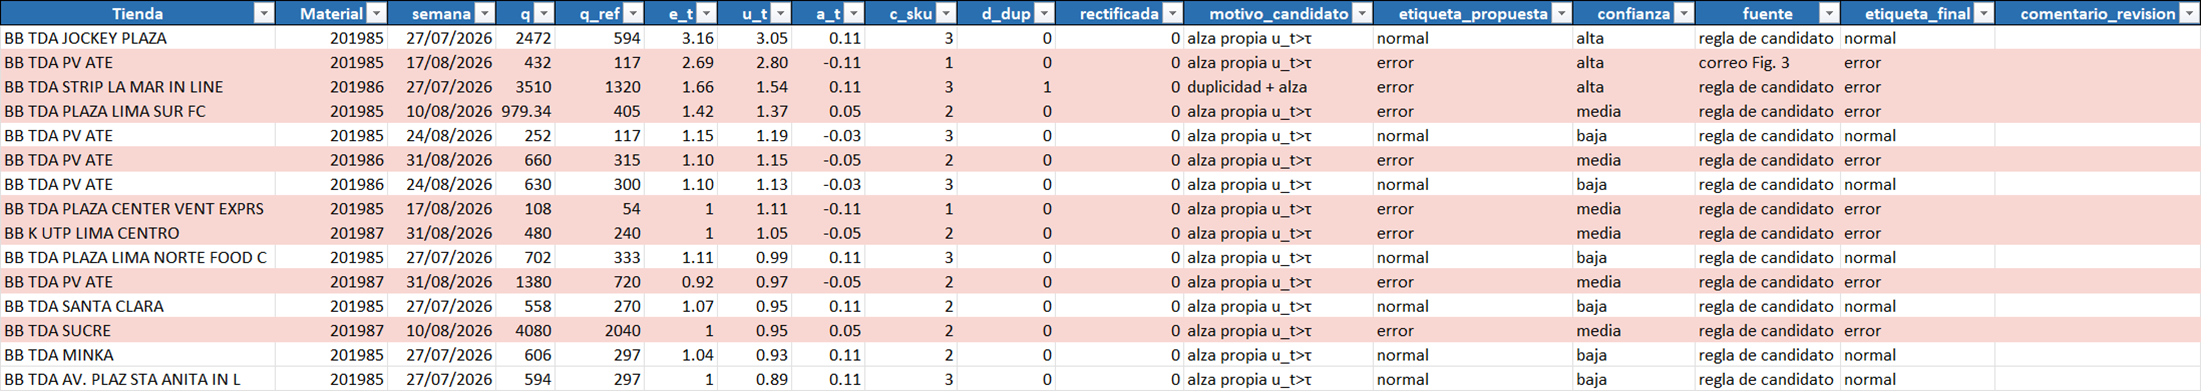
\includegraphics[width=\textwidth]{xl_03_marcado.png}
\caption{Hoja de revisión \texttt{salidas/03\_marcado.xlsx}. Cada fila es un caso sospechoso con su motivo, lo habitual de la tienda y los identificadores de sus líneas. En rojo, los casos propuestos como posible error; en la columna \texttt{etiqueta} la autora escribe \emph{error}, \emph{normal} o \emph{duda}, y en \texttt{evidencia}, la fuente. El caso C11 (ATE) ya figura como error confirmado.}
\label{fig:av-cap-marcado}
\end{figure}

La autora valida cada caso y lo marca como error solo si cuenta con alguna de estas evidencias, como un correo en que el área o la tienda reconozca el error, una corrección del pedido con su motivo o la confirmación de la analista que atendió el caso. Los casos sin evidencia quedan como «duda» y no se usan para entrenar ni para evaluar. La forma de registrar estas etiquetas se describe en la Sección~\ref{sec:etiqueta}.

En el primer entregable se propuso usar como ejemplos de error las líneas que compras anuló y volvió a cargar con otra cantidad. Esta idea se descartó. Como indicó el asesor, cambiar una cantidad puede ser una decisión legítima de la tienda. Además, en 19 de las 23 líneas la cantidad corregida es mayor que la original (por ejemplo, de 18 a 72 unidades), lo que puede deberse tanto a un error de digitación como a que la tienda decidió pedir más. Estas líneas se tratarán como casos sospechosos que requieren evidencia.

También se observó que ninguna de estas correcciones sobresale en el total semanal, porque afectan a una sola línea. Por eso se agregó la comparación por línea descrita en la Sección~\ref{sec:av-pedido}.

\subsection{Paso 4: reglas sencillas como referencia}
\label{sec:av-reglas}

Antes de entrenar el árbol de decisión se programaron tres reglas sencillas, que sirven de referencia para comparar el árbol.

\begin{enumerate}[label=\textbf{R\arabic*.}]
\item Semana anterior. Alerta si el pedido duplica el de la semana previa. Es lo más parecido a lo que hoy hace la analista.
\item Habitual de la tienda. Alerta si el pedido se aleja de lo que la tienda suele pedir más de lo que normalmente varía.
\item Inusual sin ejemplos. Es un método llamado Isolation Forest \cite{liu2008}, que no usa las etiquetas. Construye muchos árboles que parten los datos al azar y mide cuántas divisiones hacen falta para dejar aislado cada pedido. Un pedido muy distinto del resto queda aislado con pocas divisiones y se marca como inusual. Su limitación es que detecta lo \emph{raro}, no lo \emph{erróneo}, ya que una tienda grande o una semana de feriado también son raras sin ser errores.
\end{enumerate}

Las dos primeras reglas usan umbrales fijos y la tercera se ajustó con el periodo de ajuste. Como todavía hay un solo error confirmado, en esta etapa no se reporta su precisión, porque con tan pocos casos la cifra no sería concluyente. Se analizan, en cambio, dos aspectos que no dependen de las etiquetas, es decir, cuántas alertas emite cada regla por semana (Figura~\ref{fig:av-alertas}) y cómo se comporta frente a dos casos conocidos (Sección~\ref{sec:av-casos}).

\begin{figure}[htbp]
\centering
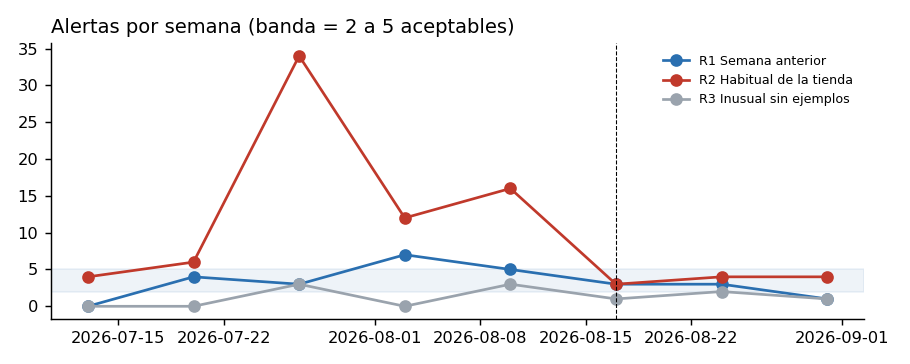
\includegraphics[width=0.85\textwidth]{fig_06_alertas_semana.png}
\caption{Número de alertas por semana de cada regla. La franja sombreada marca el volumen que el analista puede revisar; las líneas verticales marcan el inicio de la validación y de la prueba.}
\label{fig:av-alertas}
\end{figure}

La regla de la semana anterior y la del método sin ejemplos se mantienen casi siempre dentro de la franja revisable. La regla de lo habitual de la tienda emite más alertas, y en la semana de Fiestas Patrias llega a 34, porque no diferencia una tienda que sube sola de toda la cadena subiendo por el feriado. El árbol de decisión podría corregir esto, ya que dispone de la señal de movimiento común.

\subsection{Primera versión por pedido}
\label{sec:av-por-pedido}

Se programó una primera versión que evalúa cada línea en el momento de su registro, con las tres comparaciones de la Sección~\ref{sec:av-pedido}. Cada línea se compara solo con las semanas anteriores y con las líneas de la misma semana ya registradas. Los umbrales se fijaron con el periodo de ajuste, buscando unas cuatro alertas por semana. Con ellos, la comparación del acumulado de la semana emitió 4,0 alertas por semana en ese periodo, la del tamaño de la línea 3,3 y la combinación de ambas con la línea duplicada 13,5.

\begin{figure}[htbp]
\centering
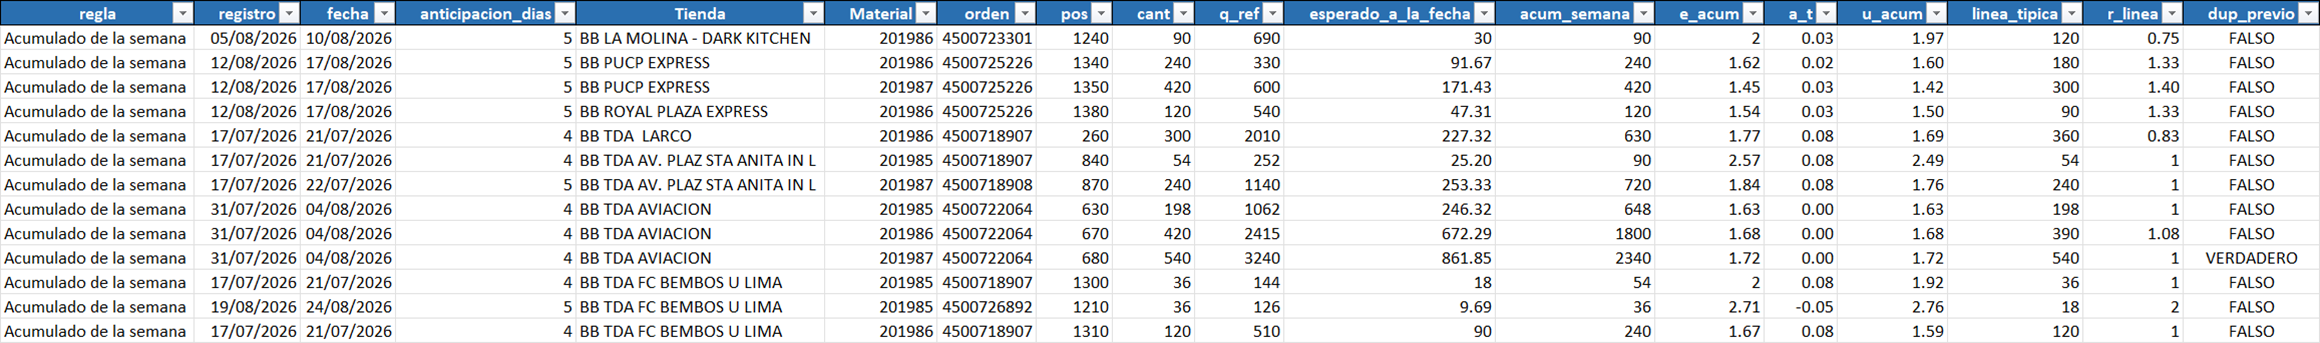
\includegraphics[width=\textwidth]{xl_05_alertas.png}
\caption{Captura de la hoja \texttt{alertas} de \texttt{salidas/05\_alertas\_pedido.xlsx}. Cada fila es una alerta emitida en la primera línea que la dispara, con su fecha de registro, su fecha de entrega y los días de anticipación.}
\label{fig:xl-alertas}
\end{figure}

Como cada alerta se emite cuando se registra la línea, también se conoce con cuánta anticipación llega. En el caso de ATE, la línea de 396 unidades se registró el 19 de agosto para entregarse el 22, y la alerta se habría emitido tres días antes del despacho.

\subsection{Primer entrenamiento del árbol y análisis de parámetros}
\label{sec:av-arbol}

Con las señales por línea y las etiquetas propuestas se entrenó una primera versión del árbol, conectada a la ventana descrita en la Sección~\ref{sec:arquitectura}. Para analizar el efecto de sus parámetros se entrenaron 24 combinaciones con el periodo de ajuste y se comparó cuántas alertas emite cada una y con qué precisión. La Tabla~\ref{tab:av-parametros} muestra las más representativas.

\begin{table}[htbp]
\centering
\caption{Análisis de parámetros del árbol entrenado con el periodo de ajuste (33 líneas de error entre 3\,902). Las alertas se cuentan por tienda, producto y semana.}
\label{tab:av-parametros}
\small
\begin{tabular}{@{}lcccc@{}}
\toprule
\textbf{Peso de la clase error} & \textbf{Profundidad} & \textbf{Hojas} & \textbf{Alertas por semana} & \textbf{Precisión} \\
\midrule
Balanceado & 2 & 4 & 42,5 & 2\,\% \\
Balanceado & 5 & 9 & 37,8 & 3\,\% \\
1 (sin ajuste) & 2 a 5 & 4 a 9 & 1,0 & 75\,\% \\
\textbf{5} & \textbf{4} & \textbf{7} & \textbf{1,8} & \textbf{57\,\%} \\
5 (mín. 20 líneas por hoja) & 4 & 5 & 7,5 & 13\,\% \\
\bottomrule
\end{tabular}
\end{table}

La tabla muestra el efecto de cada parámetro. Con el peso balanceado, que iguala la importancia total de errores y normales, el árbol emite unas 40 alertas por semana, demasiadas para revisarlas. Sin ajuste de peso ocurre lo contrario, ya que casi no alerta. Con un peso de 5 y profundidad 4 la carga baja a menos de 2 alertas por semana con 57\,\% de precisión en ajuste. Exigir al menos 20 líneas por hoja vuelve las reglas más generales, pero sube la carga y baja la precisión.

Como en el periodo de ajuste hay solo 4 casos de error, estas cifras describen cómo responde el árbol a cada parámetro, pero todavía no sirven para elegir el mejor por su capacidad de detectar errores nuevos. Por eso los parámetros se fijaron con dos criterios, una carga de alertas revisable y reglas fáciles de leer (profundidad 4, mínimo 5 líneas por hoja y peso 5 para la clase error). Con esos parámetros, el árbol se entrenó con los periodos de ajuste y validación; el periodo de prueba quedó reservado.

\begin{figure}[htbp]
\centering
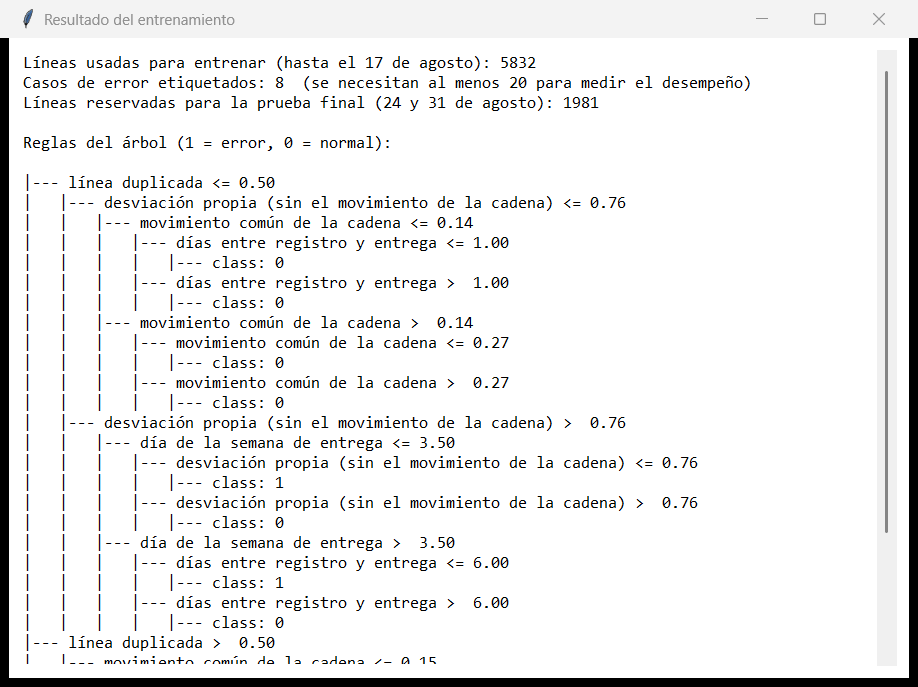
\includegraphics[width=0.75\textwidth]{app_entrenar.png}
\caption{Ventana de entrenamiento del prototipo, con los datos usados, cantidad de errores etiquetados y reglas aprendidas por el árbol.}
\label{fig:app-entrenar}
\end{figure}

\begin{figure}[htbp]
\centering

\includegraphics[width=\textwidth]{app_revisar.png}
\caption{Ventana de revisión del prototipo, con las líneas marcadas por el árbol en las últimas semanas del extracto, con su nivel, la probabilidad de la hoja y la regla en palabras.}
\label{fig:app-revisar}
\end{figure}

\subsection{Prueba con casos conocidos}
\label{sec:av-casos}

Mientras no haya suficientes errores confirmados, los métodos se prueban con dos casos cuyo resultado se conoce de antemano y que el primer entregable ya comparó en la Tabla~\ref{tab:firma}.

\begin{itemize}
\item \textbf{ATE, semana del 17 de agosto}. Es un error confirmado por correo. Un buen método \emph{debe} alertar.
\item \textbf{Fiestas Patrias, semana del 27 de julio}. Es un alza de toda la cadena, que no es error. Un buen método \emph{no debe} llenarse de alertas; esa semana hay 169 combinaciones de tienda y producto.
\end{itemize}

Para que la prueba sea justa, el árbol se entrenó sin el caso que se evalúa, es decir, sin la semana de ATE para ver si la detecta, y sin la semana de Fiestas Patrias para contar sus alertas. La Tabla~\ref{tab:av-casos} resume el resultado.

\begin{table}[htbp]
\centering
\caption{Prueba con casos conocidos. En Fiestas Patrias se cuentan las alertas emitidas, que en ese caso son falsas alarmas.}
\label{tab:av-casos}
\small
\begin{tabularx}{\textwidth}{@{}Ycc@{}}
\toprule
\textbf{Método} & \textbf{ATE, 17 de agosto (debe alertar)} & \textbf{Fiestas Patrias (alertas)} \\
\midrule
R1. Semana anterior & Sí & 3 \\
R2. Habitual de la tienda & Sí & 34 \\
R3. Inusual sin ejemplos & Sí & 3 \\
\midrule
Por pedido, acumulado de la semana & \textbf{Sí, 3 días antes} & \textbf{0} \\
Por pedido, tamaño de la línea & Sí, 3 días antes & 9 \\
Por pedido, cualquiera o línea duplicada & Sí, 3 días antes & 16 \\
\midrule
Árbol de decisión (sin haber visto el caso) & No & 3 \\
\bottomrule
\end{tabularx}
\end{table}

La comparación del acumulado de la semana es la única que cumple ambas condiciones, ya que detecta el error de ATE tres días antes de la entrega y no emite ninguna alerta en Fiestas Patrias, porque descuenta el movimiento común de la cadena. La regla de lo habitual de la tienda detecta ATE, pero se llena de falsas alarmas en el feriado. El árbol, en cambio, distingue bien el feriado, pero no reconoce el caso de ATE cuando no lo vio durante el entrenamiento. Esto confirma que, con los pocos errores etiquetados que hay hoy, el árbol todavía no aprende un patrón que pueda aplicar a casos nuevos.

\subsection{Qué hace falta para medir el desempeño}
\label{sec:av-mejoras}

La precisión y la exhaustividad, que son las metas del proyecto, se medirán una sola vez en el periodo de prueba (24 y 31 de agosto), que quedó reservado. Hacerlo hoy no sería concluyente por tres razones. Hay un solo error confirmado. En esas dos semanas hay apenas 5 casos propuestos, de modo que cada acierto movería el resultado 20 puntos. Además, las etiquetas propuestas fueron definidas por el mismo programa. Para que esa medición sea válida hace falta lo siguiente, en este orden.

\begin{enumerate}
\item \textbf{Ampliar el historial} con el extracto posterior al 11 de septiembre y, si es posible, con meses anteriores a julio, para tener más casos de error de los cuales aprender y con los cuales evaluar.
\item \textbf{Medir la versión por pedido contra etiquetas por línea}, que es la forma en que esa versión emite sus alertas.
\item \textbf{Combinar la regla de lo habitual con el filtro de campaña y de presentaciones}, y dar al árbol esa medida como una variable más, para que pueda aprovechar lo que hoy hace bien cada método.
\end{enumerate}

Ninguna de estas mejoras se ajustará mirando el periodo de prueba, para que su resultado siga siendo una medición independiente.

\iffinal\else
\subsection{Riesgos observados durante la ejecución}
\label{sec:av-riesgos}

La ejecución de estas semanas y la revisión del asesor permitieron actualizar los riesgos de la Tabla~\ref{tab:riesgos} (Tabla~\ref{tab:av-riesgos}). La responsable de todas las respuestas es la autora del proyecto.

\begin{table}[htbp]
\centering
\caption{Riesgos actualizados al cierre de la semana 6.}
\label{tab:av-riesgos}
\small
\begin{tabularx}{\textwidth}{@{}L{3.6cm}L{3.2cm}L{1.6cm}Y@{}}
\toprule
\textbf{Riesgo} & \textbf{Señal observada} & \textbf{Estado} & \textbf{Respuesta} \\
\midrule
Si no se reúnen suficientes errores confirmados, el modelo no tendrá de qué aprender & Un solo error confirmado por escrito & Ocurriendo & Revisar los 78 casos contra los correos en la semana 7; si no se alcanzan 20, reportar el método como apoyo a la revisión y no como clasificador \\
Si el modelo usa información que no existe al alertar, su desempeño real será menor que el medido & Variables calculadas sobre semanas completas & Identificado & Recalcular las señales con lo registrado hasta cada momento (Sección~\ref{sec:av-pedido}) \\
Si las etiquetas se construyen con la misma idea que una regla, esa regla parecerá mejor de lo que es & La segunda regla rinde mucho más en validación que en ajuste & Vigente & Basar la etiqueta final en evidencia operativa, no en la regla \\
Si no se obtiene un extracto posterior, no habrá periodo de prueba independiente & El extracto actual termina el 11 de septiembre & Nuevo & Solicitar el extracto de septiembre y octubre al área de planeamiento en la semana 7 \\
Si la semana del 13 de julio no fue una campaña, el método podría silenciar errores en semanas similares & Movimiento conjunto sin feriado conocido & Nuevo & Consultar por escrito al área de planeamiento \\
\bottomrule
\end{tabularx}
\end{table}

\subsection{Plan para las semanas 7 a 9}
\label{sec:av-plan}

Los hitos del plan general se mantienen, pero las tareas de las próximas semanas se ajustan para responder a la retroalimentación (Tabla~\ref{tab:av-plan}).

\begin{table}[htbp]
\centering
\caption{Tareas de las semanas 7 a 9 y sus dependencias.}
\label{tab:av-plan}
\small
\begin{tabularx}{\textwidth}{@{}cYcL{3cm}c@{}}
\toprule
& \textbf{Tarea} & \textbf{Días} & \textbf{Requiere terminar antes} & \textbf{Semana} \\
\midrule
A & Solicitar el extracto posterior al 11 de septiembre & 1 & -- & 7 \\
B & Revisar los 78 casos sospechosos contra los correos y registrar la evidencia & 3 & -- & 7 \\
C & Recalcular las señales con la información disponible en cada momento y añadir la comparación por línea & 3 & -- & 7 \\
D & Entrenar el árbol y compararlo con la mejor regla en validación & 2 & B y C & 8 \\
\multicolumn{5}{@{}l}{\quad\textit{Hito: decidir si el árbol se justifica. Decide la autora con el visto bueno del asesor.}} \\
E & Elegir a partir de qué desviación se emite una alerta y redactar los motivos & 2 & D & 8 \\
F & Construir el motor de cálculo que evalúa cada línea registrada & 4 & E & 9 \\
G & Evaluar una sola vez sobre el extracto independiente & 1 & A y F & 9 \\
\bottomrule
\end{tabularx}
\end{table}

Respecto del plan original, el hito del paso 5 se desplaza de la semana 7 a la 8, porque la revisión con evidencia y el recálculo de las señales deben completarse antes de entrenar el árbol. Este desplazamiento se absorbe dentro de la semana 8 y no afecta la entrega de la semana 12. La dependencia más frágil es la revisión de casos (B), porque depende de los correos que conserva el área de planeamiento; si se retrasa, la elección del umbral (E) se simplificará comparando solo tres valores posibles.

\fi

\begin{thebibliography}{99}

\bibitem{aggarwal2017} Charu C. Aggarwal. \emph{Outlier Analysis}. Springer, 2nd edition, 2017.

\bibitem{ambler2023} Scott W. Ambler and Mark Lines. \emph{¡Elija su WoW! Un enfoque de Disciplined Agile para optimizar su forma de trabajar}. Project Management Institute, 2.\textsuperscript{a} edition, 2023.

\bibitem{breiman1984} Leo Breiman, Jerome H. Friedman, Richard A. Olshen, and Charles J. Stone. \emph{Classification and Regression Trees}. Wadsworth and Brooks/Cole, Monterey, CA, 1984.

\bibitem{chandola2009} Varun Chandola, Arindam Banerjee, and Vipin Kumar. Anomaly detection: A survey. \emph{ACM Computing Surveys}, 41(3):15:1--15:58, 2009. Artículo 15.

\bibitem{chen2016} Tianqi Chen and Carlos Guestrin. XGBoost: A scalable tree boosting system. In \emph{Proceedings of the 22nd ACM SIGKDD International Conference on Knowledge Discovery and Data Mining}, pages 785--794, 2016.

\bibitem{hodge2004} Victoria J. Hodge and Jim Austin. A survey of outlier detection methodologies. \emph{Artificial Intelligence Review}, 22(2):85--126, 2004.

\bibitem{hyndman2021} Rob J. Hyndman and George Athanasopoulos. \emph{Forecasting: Principles and Practice}. OTexts, Melbourne, Australia, 3rd edition, 2021. \url{https://otexts.com/fpp3/}.

\bibitem{ishikawa} Kaoru Ishikawa. \emph{Guide to Quality Control}. Asian Productivity Organization, Tokio, 2nd edition, 1986.

\bibitem{lee1997} Hau L. Lee, V. Padmanabhan, and Seungjin Whang. Information distortion in a supply chain: The bullwhip effect. \emph{Management Science}, 43(4):546--558, 1997.

\bibitem{liu2008} Fei Tony Liu, Kai Ming Ting, and Zhi-Hua Zhou. Isolation forest. In \emph{Proceedings of the 8th IEEE International Conference on Data Mining (ICDM)}, pages 413--422. IEEE, 2008.

\bibitem{lundberg2017} Scott M. Lundberg and Su-In Lee. A unified approach to interpreting model predictions. In \emph{Advances in Neural Information Processing Systems (NeurIPS)}, volume 30, pages 4765--4774, 2017.

\bibitem{pedregosa2011} Fabian Pedregosa, Gaël Varoquaux, Alexandre Gramfort, Vincent Michel, Bertrand Thirion, Olivier Grisel, Mathieu Blondel, Peter Prettenhofer, Ron Weiss, Vincent Dubourg, Jake Vanderplas, Alexandre Passos, David Cournapeau, Matthieu Brucher, Matthieu Perrot, and Édouard Duchesnay. Scikit-learn: Machine learning in Python. \emph{Journal of Machine Learning Research}, 12:2825--2830, 2011.

\bibitem{pmbok2025} Project Management Institute. \emph{The Standard for Project Management and A Guide to the Project Management Body of Knowledge (PMBOK Guide)}. Project Management Institute, Newtown Square, PA, 8th edition, 2025.

\bibitem{quinlan1993} J. Ross Quinlan. \emph{C4.5: Programs for Machine Learning}. Morgan Kaufmann, San Mateo, CA, 1993.

\bibitem{wirth2000} Rüdiger Wirth and Jochen Hipp. CRISP-DM: Towards a standard process model for data mining. \emph{Proceedings of the 4th International Conference on the Practical Application of Knowledge Discovery and Data Mining}, pages 29--39, 2000.

\end{thebibliography}

\appendix
% ============================================================
%  Anexo: evidencias del prototipo (capturas de Excel y del código)
% ============================================================

\section{Evidencias del prototipo}
\label{sec:anexo}

Este anexo documenta el prototipo construido en las semanas 1 a 6. Para cada paso se muestra el archivo de Excel que produce, tal como lo vería la analista de planeamiento, y la función del programa que lo genera. El prototipo se ejecuta con dos órdenes sobre el archivo exportado del sistema de compras, sin modificarlo:

\begin{center}
\texttt{python src/pipeline.py exportBIMBO.XLSX}\\
\texttt{python src/pedido.py exportBIMBO.XLSX [extracto\_de\_prueba.xlsx]}
\end{center}

\begin{table}[H]
\centering
\caption{Organización del prototipo.}
\label{tab:repo}
\small
\begin{tabularx}{\textwidth}{@{}L{4.2cm}Y@{}}
\toprule
\textbf{Archivo} & \textbf{Función} \\
\midrule
\texttt{src/pipeline.py} & Pasos 1 a 4 en su versión semanal: limpieza, señales, casos sospechosos y reglas sencillas \\
\texttt{src/pedido.py} & Versión por pedido: señales con la información disponible al registrar cada línea, umbrales calibrados en el periodo de ajuste y métricas por periodo \\
\texttt{src/figuras\_gestion.py} & EDT, diagrama de Gantt y matriz de riesgos \\
\texttt{src/capturas\_excel.ps1}, \texttt{src/capturas\_codigo.py} & Generan las capturas de este anexo \\
\texttt{salidas/01} a \texttt{05\_*.xlsx} & Archivos de resultados de cada paso \\
\bottomrule
\end{tabularx}
\end{table}

\subsection{Archivo de entrada}

\begin{figure}[H]
\centering
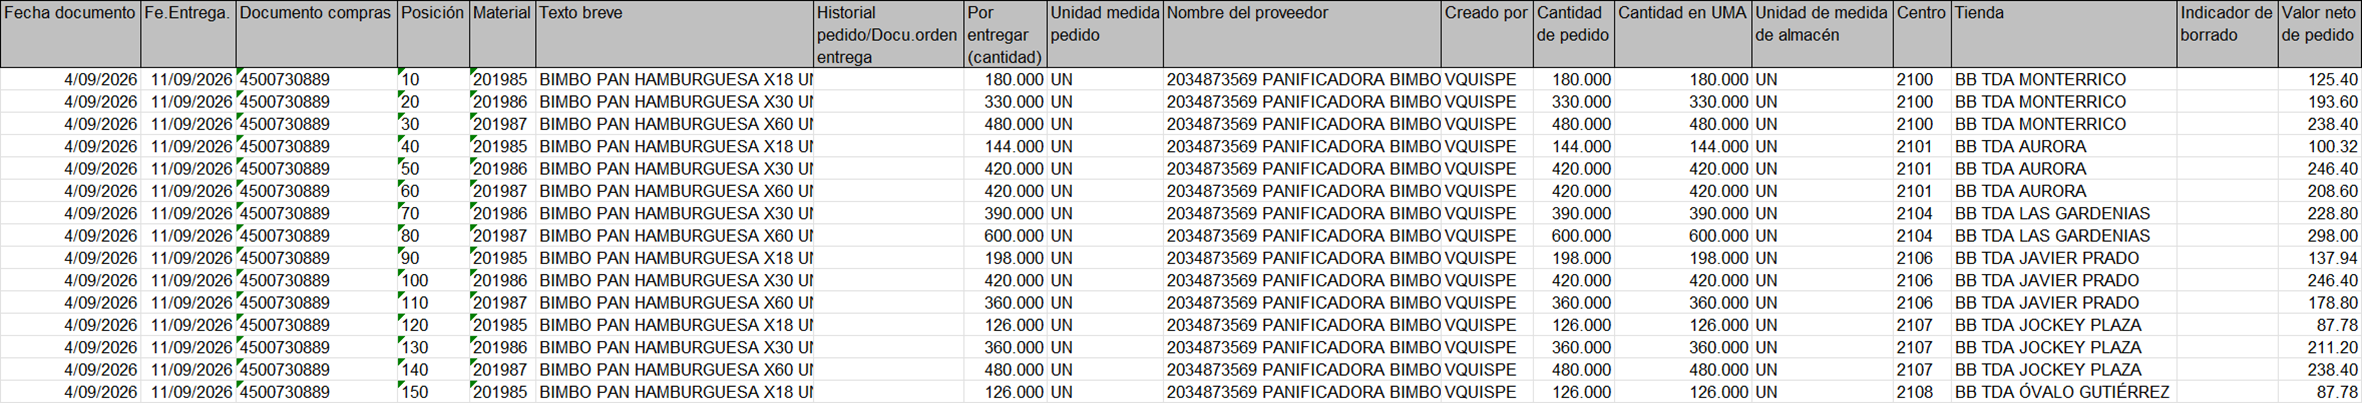
\includegraphics[width=\textwidth]{xl_00_original.png}
\caption{Archivo \texttt{exportBIMBO.xlsx} tal como se exporta del sistema de compras. Es la única entrada del prototipo.}
\label{fig:xl-original}
\end{figure}

\subsection{Paso 1: limpieza}

\begin{figure}[H]
\centering
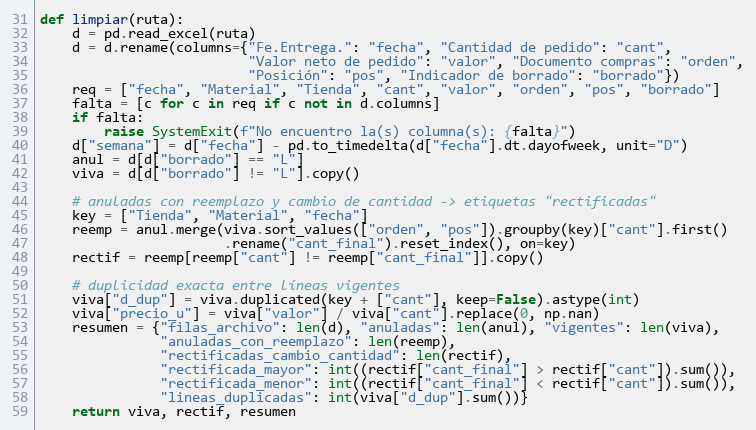
\includegraphics[width=0.85\textwidth]{code_01_limpiar.png}
\caption{Función \texttt{limpiar} (\texttt{src/pipeline.py}): verifica las columnas, separa las líneas anuladas, empareja cada anulada con su reemplazo y marca los duplicados.}
\label{fig:code-limpiar}
\end{figure}

\begin{figure}[H]
\centering
\begin{minipage}[t]{0.32\textwidth}\centering
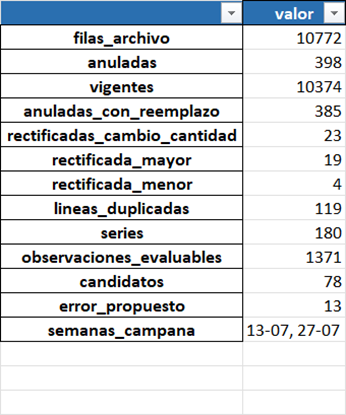
\includegraphics[width=\textwidth]{xl_01_resumen.png}
\end{minipage}\hfill
\begin{minipage}[t]{0.66\textwidth}\centering
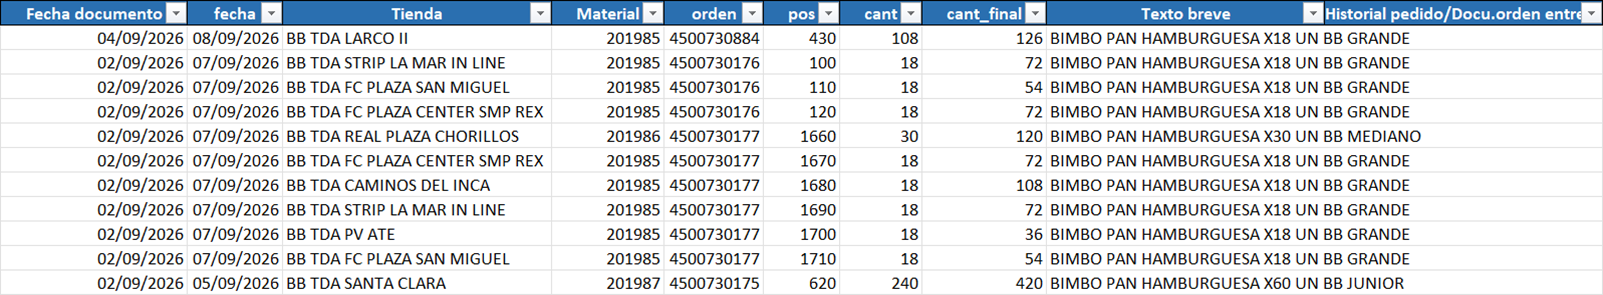
\includegraphics[width=\textwidth]{xl_01_rectificadas.png}
\end{minipage}
\caption{\texttt{salidas/01\_limpio.xlsx}. A la izquierda, la hoja \texttt{resumen} con las cifras de limpieza; a la derecha, la hoja \texttt{rectificadas} con las líneas anuladas cuya cantidad cambió.}
\label{fig:xl-limpio}
\end{figure}

\subsection{Paso 2: señales}

\begin{figure}[H]
\centering
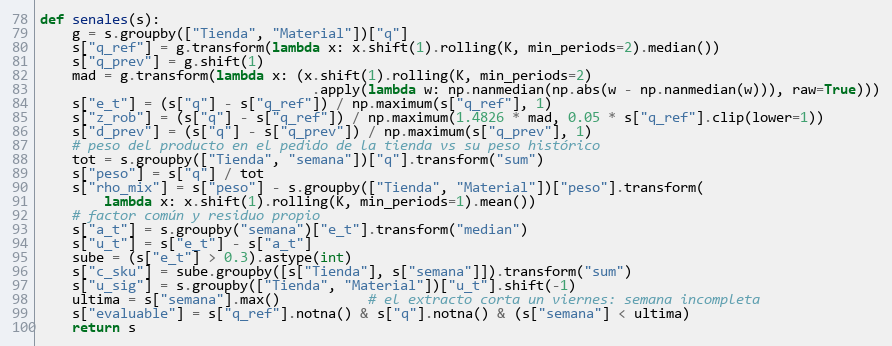
\includegraphics[width=0.9\textwidth]{code_02_senales.png}
\caption{Función \texttt{senales} (\texttt{src/pipeline.py}): referencia de la tienda, desviación, variación semanal, peso del producto, movimiento común de la cadena y presentaciones en alza. El resultado se muestra en la Figura~\ref{fig:av-cap-senales}.}
\label{fig:code-senales}
\end{figure}

\subsection{Paso 3: casos sospechosos}

\begin{figure}[H]
\centering
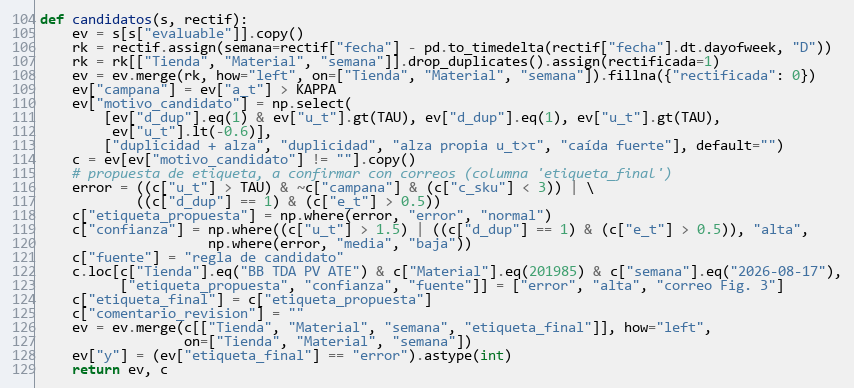
\includegraphics[width=0.9\textwidth]{code_03_candidatos.png}
\caption{Función \texttt{candidatos} (\texttt{src/pipeline.py}): selecciona los casos sospechosos, propone una etiqueta con su regla explícita y deja las columnas para la revisión con evidencia. El resultado se muestra en la Figura~\ref{fig:av-cap-marcado}.}
\label{fig:code-candidatos}
\end{figure}

\subsection{Paso 4: reglas sencillas}

\begin{figure}[H]
\centering
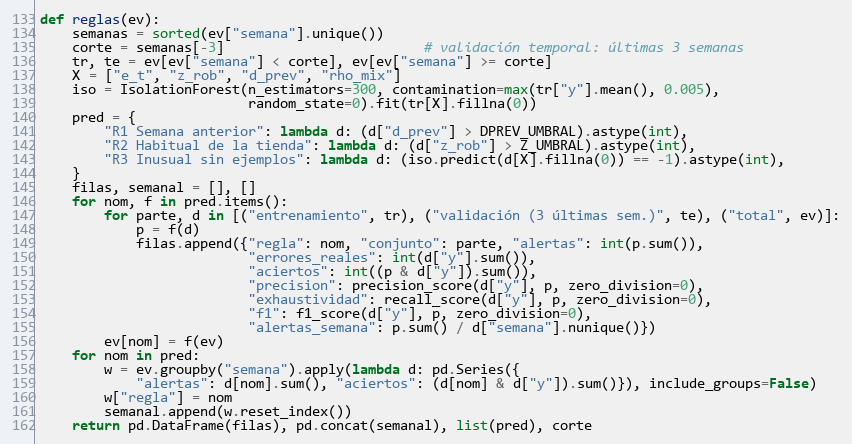
\includegraphics[width=0.9\textwidth]{code_04_reglas.png}
\caption{Función \texttt{reglas} (\texttt{src/pipeline.py}): separa el periodo de ajuste del de validación y calcula, para cada regla, alertas, aciertos, precisión y exhaustividad.}
\label{fig:code-reglas}
\end{figure}

\begin{figure}[H]
\centering
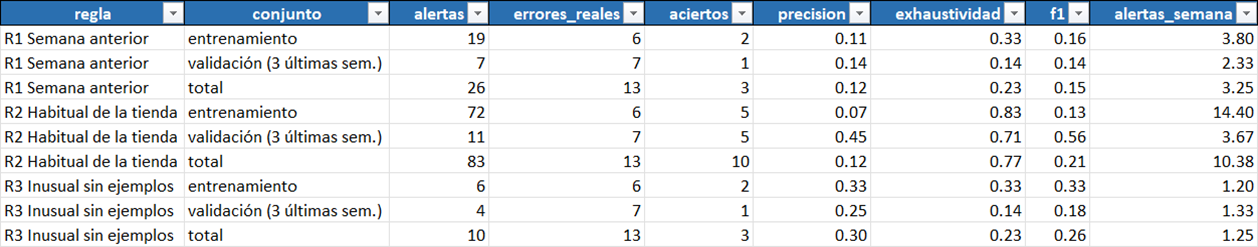
\includegraphics[width=0.8\textwidth]{xl_04_metricas.png}
\caption{Hoja \texttt{metricas} de \texttt{salidas/04\_reglas.xlsx}, origen de la Tabla~\ref{tab:av-reglas}.}
\label{fig:xl-reglas}
\end{figure}

\subsection{Versión por pedido}

\begin{figure}[H]
\centering
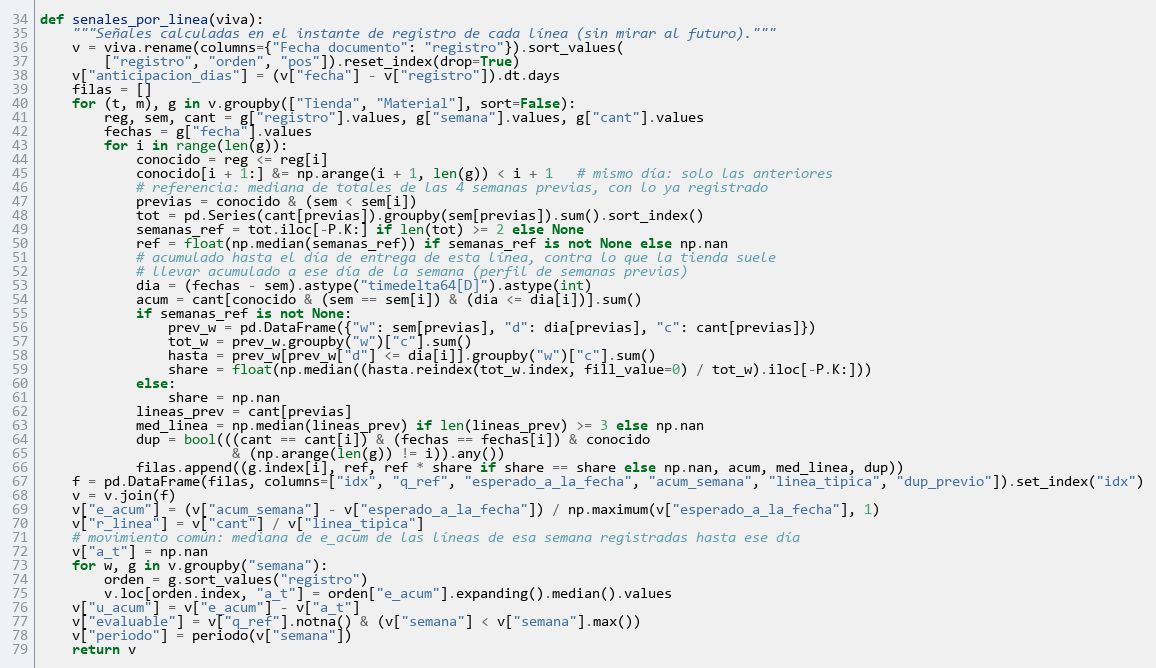
\includegraphics[width=0.9\textwidth]{code_05_por_linea.png}
\caption{Función \texttt{senales\_por\_linea} (\texttt{src/pedido.py}): para cada línea usa solo lo registrado hasta ese día. La referencia sale de semanas anteriores y el acumulado se compara con lo que la tienda suele llevar a esa fecha.}
\label{fig:code-linea}
\end{figure}

\begin{figure}[H]
\centering
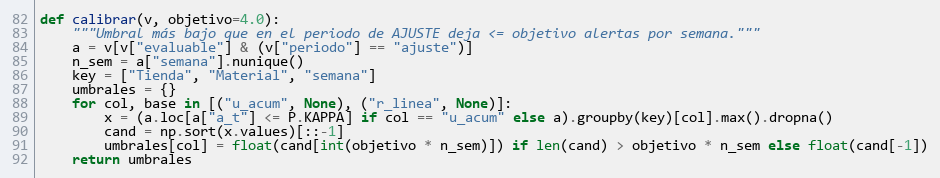
\includegraphics[width=0.75\textwidth]{code_06_calibrar.png}
\caption{Función \texttt{calibrar} (\texttt{src/pedido.py}): fija los umbrales solo con el periodo de ajuste, para unas cuatro alertas por semana.}
\label{fig:code-calibrar}
\end{figure}

\begin{figure}[H]
\centering
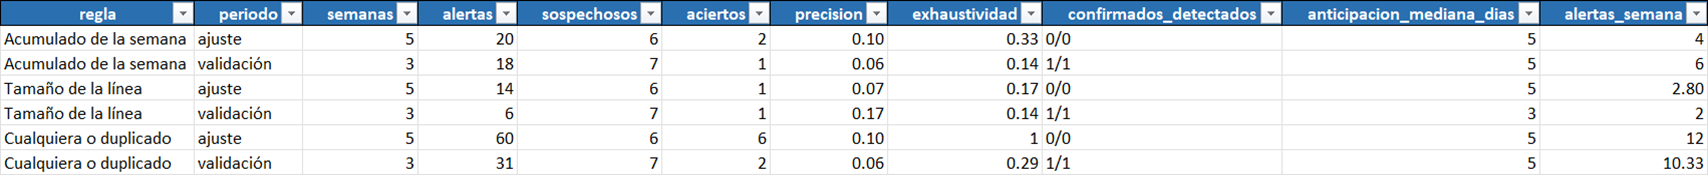
\includegraphics[width=\textwidth]{xl_05_metricas_pedido.png}
\caption{Hoja \texttt{metricas\_por\_periodo} de \texttt{salidas/05\_alertas\_pedido.xlsx}, origen de la Tabla~\ref{tab:av-pedido}. La columna \texttt{confirmados\_detectados} muestra que el caso ATE se detecta en validación.}
\label{fig:xl-pedido}
\end{figure}

\end{document}
